\documentclass[11pt,a4paper]{article}

\usepackage[utf8]{inputenc}
\usepackage[T1]{fontenc}
\usepackage[english]{babel}
\usepackage{lmodern}
\usepackage{geometry}
\geometry{margin=2.5cm}
\usepackage{amsmath,amssymb,amsthm,mathtools}
\usepackage{enumitem}
\usepackage{microtype}
\usepackage{xcolor}
\usepackage{bm}
\usepackage{float}
\usepackage{graphicx}
\usepackage{caption}
\usepackage{subcaption}
\usepackage{booktabs}
\usepackage{array}
\usepackage{algorithm}
\usepackage{algpseudocode}
\usepackage{listings}
\usepackage{inconsolata}
\usepackage{xurl}

\graphicspath{{figures/}}

\usepackage[colorlinks=true,linkcolor=blue,citecolor=red,urlcolor=magenta]{hyperref}

\newcommand{\email}[1]{\texttt{\small \href{mailto:#1}{#1}}} % Small font email command

\definecolor{codebg}{RGB}{248,248,248}
\definecolor{codeframe}{RGB}{220,220,220}
\definecolor{comment}{RGB}{0,102,0}
\definecolor{keyword}{RGB}{0,0,150}
\definecolor{string}{RGB}{163,21,21}
\definecolor{number}{RGB}{128,0,128}
\lstdefinestyle{pyStyle}{language=Python,basicstyle=\footnotesize\ttfamily,backgroundcolor=\color{codebg},frame=single,rulecolor=\color{codeframe},frameround=tttt,framesep=6pt,xleftmargin=6pt,xrightmargin=6pt,showstringspaces=false,tabsize=4,breaklines=true,breakatwhitespace=true,captionpos=b,numbers=left,numberstyle=\scriptsize\color{number},numbersep=8pt,keywordstyle=\bfseries\color{keyword},commentstyle=\itshape\color{comment},stringstyle=\color{string},upquote=true}

\newtheorem{theorem}{Theorem}[section]
\newtheorem{lemma}[theorem]{Lemma}
\newtheorem{proposition}[theorem]{Proposition}
\newtheorem{corollary}[theorem]{Corollary}
%\theoremstyle{definition}
\newtheorem{definition}[theorem]{Definition}
\newtheorem{example}[theorem]{Example}
\newtheorem{remark}[theorem]{Remark}

\newcommand{\NS}{\mathsf{NS}}
\newcommand{\nstriple}[1]{\langle #1 \rangle}
\newcommand{\turiyam}[1]{\langle #1 \rangle_{\mathsf{Tuy}}}
\newcommand{\R}{\mathbb{R}}
\newcommand{\N}{\mathbb{N}}
\newcommand{\score}{\mathrm{Sc}}
\newcommand{\Score}[2][]{\score_{#1}\!\left(#2\right)}
\newcommand{\ScoreL}[1]{\Score[\lambda]{#1}}
\newcommand{\Trust}{\mathsf{Tr}}
\newcommand{\Bel}{\mathrm{Bel}}
\newcommand{\Pl}{\mathrm{Pl}}
\newcommand{\Act}{\mathcal{A}}
\DeclareMathOperator*{\argmax}{arg\,max}
\DeclareMathOperator*{\argmin}{arg\,min}
\newcommand{\Sc}{\operatorname{Sc}}

\newcommand{\ds}{\displaystyle}

\title{\textbf{A Neutrosophic Agent-Based Network Model for Immigration and Coexistence}}
\author{Giorgio Nordo$^{1}$ \and Carmelo Filippo Munaf\`o$^{1,2,3,*}$ \and Nivetha Martin$^{4}$}
\date{}

\begin{document}
	\maketitle
	
	\begin{center}
\small
$^1$ Department of Mathematical and Computer Sciences, Physical Sciences and Earth Sciences,\\
University of Messina, Viale Ferdinando Stagno d'Alcontres 31, 98166 Messina, Italy\\
\email{giorgio.nordo@unime.it}\\[1mm]
$^2$ Department of Industrial Engineering, University of Salerno, Fisciano, Italy\\
$^3$ Department for the Promotion of Human Science and Quality of Life, San Raffaele University, Rome, Italy\\
\email{carmelofilippo.munafo@unime.it}\\[1mm]
$^4$ Department of Mathematics, Arul Anandar College (Autonomous), Karumathur, Madurai, Tamil Nadu 625514, India;\\
Dean of Research Institute, Arul Anandar College (Autonomous)\\
\email{nivetha.martin710@gmail.com}\\[2mm]
\textbf{Author identifiers:}\\
Giorgio Nordo, ORCID \href{https://orcid.org/0000-0002-9585-9680}{0000-0002-9585-9680};\\
Carmelo Filippo Munaf\`o, ORCID \href{https://orcid.org/0000-0003-3611-0941}{0000-0003-3611-0941};\\
Nivetha Martin, ORCID \href{https://orcid.org/0000-0001-9942-1320}{0000-0001-9942-1320}, Scopus Author ID 56939762600,\\
ResearchGate: \url{https://www.researchgate.net/profile/Nivetha-Martin}\\[2mm]
$^{*}$ Corresponding author: \email{carmelofilippo.munafo@unime.it}
\end{center}
	
	%--------------------------------------------------------------------------
	% ABSTRACT
	%--------------------------------------------------------------------------
	\begin{abstract}
		A single-valued neutrosophic extension of adaptive-agent-based network models for the study of host-guest interactions, in migration contexts, is proposed. Unlike the original formulation developed by D'Orsogna et al. in \cite{chuang2019}, each agent is described by a single-valued neutrosophic attitude $\nstriple{T,I,F}\in[0,1]^3$, quantifying, respectively, the propensity toward integration-oriented acceptance ($T$), indeterminacy ($I$), the propensity to reject coexistence with other groups, favoring segregation ($F$). Compared with a purely scalar attitude model, this framework separates acceptance, refusal, and undecidedness, which is crucial in migration contexts where an observed moderate position may correspond either to a genuine compromise or to unresolved ambiguity. Moreover, it captures the key characteristics of social interactions more effectively.
		The revised model improves the previous formulation in four main directions. First, the network structure is extended from the basic Erd\H{o}s--R\'enyi baseline (random network) to Watts--Strogatz small-world and Barab\'asi--Albert scale-free topologies (scale-free networks). Second, the utility function depends on the agents' capacity: agents with higher socioeconomic reward and higher neutrosophic scores can maintain more social connections without a proportional loss of effectiveness. Third, the rewiring process is refined by combining multi-agent Q-learning with a Dezert–Smarandache-inspired trust aggregation mechanism. This allows agents to learn which relations maximize long-term network profit and do not choose candidates only by pairwise similarity. 		
		Numerical simulations compare random, small-world, and scale-free networks, examine the evolution of an integration index, and reproduce neighbourhood tipping as the proportion of migrants changes.
	\end{abstract}
	
	\noindent\textbf{Keywords:} neutrosophic agent-based model; immigration; coexistence; adaptive networks; scale-free networks; small-world networks; Q-learning; DSmT;  neighbourhood tipping.
	
	%--------------------------------------------------------------------------
	% INTRODUCTION
	%--------------------------------------------------------------------------
	\section{Introduction}
	Mathematical modelling of migration and social integration phenomena has received considerable attention over the past decades, as a valuable tool for understanding the emergence of collective behaviors in heterogeneous societies. Among the pioneering contributions are the classical studies of Schelling \cite{schelling1969,schelling1971}, which demonstrated that simple local interaction rules can generate segregated global patterns. 
	More recently, agent-based models on adaptive/dynamic networks have enriched this field, by allowing both individual attitudes and social relationships to evolve over time. In particular, the immigration model proposed by Chuang, Chou, and D'Orsogna \cite{chuang2019,chuang2020} showed that the long-term outcome of host-guest interaction, namely integration or enclave formation, is strongly affected by the balance between cultural adaptation and evolution of social links.
	
	A limitation of original scalar attitude models is that each individual attitude is represented by a single numerical value. Real social processes, however, are inherently multidimensional: the same agent may simultaneously exhibit  openness toward certain cultural traits, resistance toward others, and undecidedness regarding future interactions.
	A one-dimensional variable cannot adequately capture these coexisting and potential conflicting attitudes. To overcome this limitation, in the present work we replace the one-dimensional representation of individual attitude with a three-component representation by adopting a single-valued neutrosophic representation of individual attitudes. Specifically, each agent is described by the neutrosophic state $\nstriple{T,I,F}$, where $T$ denotes integration-oriented acceptance, $F$ measures segregation-oriented rejection, and $I$ measures indeterminacy or ambivalence.
	This new attitude formulation provides a more expressive and realistic framework for describing social behavior under uncertainty while preserving computational simplicity.
	
	However, the original implementation used an Erd\H{o}s--R\'enyi graph that is useful as a statistical baseline, but it is not a realistic model of human societies, because it does not accurately reproduce the structural properties commonly observed in social networks. In fact, empirical social networks typically exhibit high clustering, short average path lengths, and sometimes hub-like individuals who concentrate social influence \cite{watts1998, barabasi1999, newman2010,barrat2008}. We improve the underlying model by replacing the purely random Erd\H{o}s--R\'enyi initialization with a Watts--Strogatz small world topology, which better reproduces the clustering and short communication patterns observed in real social networks. Then, we compare three initial topologies: Erd\H{o}s-R\'enyi, Watts--Strogatz small-world, and Barab\'asi-Albert scale-free networks. 
	
	Finally, the combination of a neutrosophic representation of attitudes with a more realistic network topology yields a richer framework for investigating migration dynamics. Besides improving the descriptive power of the original model, it enables the analysis of how uncertainty, network organization, and social influence interact in shaping collective interaction processes.

	%--------------------------------------------------------------------------
	% SECTION 2
	%--------------------------------------------------------------------------
	\section{Single-valued neutrosophic preliminaries}
	In this section, we briefly recall the main concepts of single-valued neutrosophic theory that are used throughout the paper. Introduced by Smarandache in \cite{smarandache1999} as a general framework for modeling uncertainty, indeterminacy, and inconsistency, neutrosophic sets extend both fuzzy sets and intuitionistic fuzzy sets by representing each element through three independent membership degrees: truth, indeterminacy, and falsity.
	Among the various formulations, single-valued neutrosophic sets (SVNSs), proposed by Wang et al. \cite{wang2010svns}, are particularly suitable for computational applications, since all three components take values in the interval $[0,1]$. 
	Due to their ability to simultaneously represent uncertainty, indeterminacy, and inconsistency, SVNSs have been successfully applied	in decision-making \cite{ye2014crossentropy,sodenkamp2018} and, together with the corresponding single-valued neutrosophic graph models, in social network analysis \cite{mahapatra2020,peng2022}, as well as in many other fields.
	
	For completeness, we recall definitions and operators that will be employed in the proposed model.
	
	\begin{definition}[Single-valued neutrosophic attitude]
		A \textbf{single-valued neutrosophic attitude} is a triple
		$$
		x = \nstriple{T,I,F}\in[0,1]^3,
		$$
		where $T$ is the degree of integration-oriented acceptance, $I$ is the degree of indeterminacy, and $F$ is the degree of segregation-oriented rejection. Unlike intuitionistic fuzzy sets, the three components are independent, and therefore no constraints, such $T + I + F = 1$ is required. The only admissibility conditions is that $T,F,I \in (0,1)$.
	\end{definition}
	
	\begin{definition}[Parametric score]
		Let $\lambda \in [0,1]$, the \textbf{score} of $ x = \nstriple{T,I,F}$ is defined by
		\begin{equation}\label{eq:score}
			\Score[\lambda]{x} = T - \lambda F - ( 1 - \lambda) I.
		\end{equation}
		The parameter $\lambda$ determines how the negative contribution (relative penalty) is distributed between opposition $F$ and indeterminacy $I$ while keeping the total penalty equal to one. Specifically, $\lambda$ represents the relative weight assigned to opposition $F$, whereas $1-\lambda$ is the weight assigned to indeterminacy $I$.
	\end{definition}
	
	The extreme values of $\lambda$ correspond to two limiting decision criteria. For $\lambda = 1$, the score reduces to
	$$
	\Score[1]{x} = T - F,
	$$
	so that only the balance between truth and opposition is taken into account, while indeterminacy is completely neglected. Conversely, for $\lambda = 0$,
	$$
	\Score[0]{x} = T - I,
	$$
	and the evaluation depends exclusively on the balance between truth and indeterminacy, with opposition playing no role. 
	Intermediate values $0<\lambda<1$ provide a continuous interpolation between these two criteria, allowing the decision maker to calibrate the relative importance of opposition and indeterminacy according to the application.
	
	Mathematically, the previous definition introduces a one-parameter family of linear functionals on the neutrosophic state space $[0,1]^3$. For each $\lambda\in[0,1]$, the mapping
	$$
	\lambda \quad \longmapsto \quad \Score[\lambda]{\nstriple{T,I,F}} = T - \lambda F - (1 - \lambda)I
	$$
	assigns a real value to every neutrosophic state $x = \nstriple{T,I,F}$. This value is not a distance but a \emph{scoring function}, namely, a scalar evaluation index that induces an ordering of neutrosophic states according to the chosen value of $\lambda$.

	\begin{definition}[Projection and componentwise operators]
		For $z=(z_T,z_I,z_F)\in\R^3$, define the \textbf{projection} as
		$$ 
		\Pi(z) = \nstriple{ \min\{1,\max\{0,z_T\}\}, \min\{1,\max\{0,z_I\}\}, \min\{1,\max\{0,z_F\}\}}.
		$$
		For $x,y\in[0,1]^3$, write:
		\begin{alignat*}{2}
			x \odot y &= (x_T\cdot y_T, x_I\cdot y_I, x_F\cdot y_F), &\qquad& \text{ for the componentwise product}, \\
			x \oplus y &= \Pi(x+y) &\qquad& \text{ for truncated addition} \\
			x \ominus y &= \Pi(x-y) &\qquad& \text{ for truncated subtraction}
		\end{alignat*}
	\end{definition}
	
	\medskip
	A genuine metric on neutrosophic states can be defined by means of the Hausdorff neutrosophic distance, which is introduced below. 
	However, as will be shown in Section~\ref{sec:numerical}, the numerical simulations are performed using the score distance for computational simplicity.
	
	We remember that, let $x = \nstriple{T_x,I_x,F_x}$ and $y = \nstriple{T_y,I_y,F_y}$ two neutrosophic states, the following expression 
	$$
	d_\infty(x,y) = \max\{ |T_x-T_y|,\,|I_x-I_y|,\, |F_x-F_y| \}.
	$$ 
	defines the $\ell_\infty$ metric on $[0,1]^3$.
	
	\begin{definition}[A Hausdorff-consistent neutrosophic distance]
		Let $x = \nstriple{T_x,I_x,F_x}$ and $y = \nstriple{T_y,I_y,F_y}$ two neutrosophic states. If finite populations of attitudes are represented by compact subsets 
		$$
		A,B\subset[0,1]^3
		$$ 
		the induced \textbf{Hausdorff distance} is defined by
		$$
		d_H(A,B) = \max \left\{ \sup_{a\in A} \inf_{b\in B} d(a,b),\ \sup_{b\in B}\inf_{a\in A} d(a,b) \right\}.
		$$
		where $d(\cdot,\cdot)$ denotes a metric on individual neutrosophic states (for example, the Euclidean distance). In this work we consider $d(\cdot,\cdot)=d_\infty(\cdot,\cdot)$, and we get
		\begin{equation}\label{eq:hausdorff}
			d_H(A,B) = \max \left\{ \sup_{a\in A} \inf_{b\in B} d_\infty(a,b),\ \sup_{b\in B}\inf_{a\in A} d_\infty(a,b) \right\}.
		\end{equation}
		For singleton sets $A = \{x\}$ and $B = \{y\}$, one has that the two distances, Hausdorff and $\ell_\infty$, coincide, \emph{i.e.} $d_H(A,B) = d_\infty(x,y)$. 
	\end{definition}
	
	\medskip
	The Hausdorff distance measures the greatest discrepancy between the two sets. Specifically, for each point in $A$, one considers its distance to the nearest point in $B$, and then takes the largest of these minimum distances. The same procedure is repeated with the roles of $A$ and $B$ exchanged, and the Hausdorff distance is the maximum of the two resulting quantities. Equivalently, it is the smallest radius $r$ such that every point of $A$ lies within distance $r$ of some point of $B$, and every point of $B$ lies within distance $r$ of some point of $A$.
	
	In the present framework, the Hausdorff distance provides a genuine metric between populations of neutrosophic attitudes, as it compares the entire geometric configuration of the states rather than only their scalar score values. Nevertheless, as shown in the numerical experiments, the simulations are performed using the score distance because of its significantly lower computational cost.
	
	\begin{proposition}\label{prop:hausdorff-metric}
		The function $d_H$ defined in \eqref{eq:hausdorff} is a metric on the family of non-empty compact subsets of $[0,1]^3$. In particular, $d_\infty$ is a metric on the SVNS attitude space.
		
		\begin{proof}
			The function $d_\infty$ is the standard maximum norm metric on $\mathbb{R}^3$, restricted to $[0,1]^3$. The Hausdorff construction over the family of non-empty compact subsets of a metric space defines again a metric. Indeed, non-negativity, symmetry, and the identity of indiscernibles follow directly from the corresponding properties of $d_\infty$, while compactness guarantees that the relevant infima and suprema are attained. The triangle inequality follows from the triangle inequality for $d_\infty$: for each $a\in A$, one selects a point of $B$ that is arbitrarily close to minimizing the distance from $a$, and then a point of $C$ that is arbitrarily close to minimizing the distance from that point of $B$. Taking the appropriate suprema and infima yields the desired inequality. Finally, when $A=\{x\}$ and $B=\{y\}$ are singletons, the definition immediately reduces to
			$$
			d_H(\{x\},\{y\})=d_\infty(x,y).
			$$
		\end{proof}  
	\end{proposition}
	
	For decision and rewiring, we use the \textbf{scalar score distance} defined by
	$$
	\delta_{ij}^t = \left| \Score[\lambda]{x_i^t} - \Score[\lambda]{x_j^t}\right|,
	$$
	with \textbf{similarity}
	$$
	S_{ij}^t = \exp\!\left( - \frac{(\delta_{ij}^t)^2}{2\sigma^2} \right).	
	$$
	where $\sigma>0$ represents the attitudinal sensitivity parameter. Small values of $\sigma$ make similarity decrease sharply when agents have different scores; hence they increase  the risk of social polarization by reducing the perceived  compatibility between agents with distinct neutrosophic evaluations. Larger values of $\sigma$ produce more tolerant similarity profiles.
	
	%--------------------------------------------------------------------------
	% SECTION 3
	%--------------------------------------------------------------------------
	\section{Network topology}
	
	At each discrete time $t$, let
	$$
	G^t = (V,E^t)
	$$
	be a dynamic social graph whose vertices are endowed with
	single-valued neutrosophic states, following the general framework of single-valued neutrosophic graphs introduced in
	\cite{broumi2016}.
	
	The vertex set is assumed to be constant over time and is partitioned as
	$$ V = H \,\dot{\cup}\, M_1 \,\dot{\cup}\, \cdots \,\dot{\cup}\, M_m,
	$$
	where $H$ is the set of host individuals and, for
	$r=1,\ldots,m$, $M_r$ is the set of guest or migrant individuals
	belonging to the $r$-th group. The symbol $\dot{\cup}$ emphasizes that these subsets are pairwise disjoint.
	
	The time-dependent edge set $E^t$ represents the social connections that are active at time $t$. In the undirected case,
	$$
	E^t
	\subseteq \bigl\{\{i,j\}:i,j\in V,\ i\neq j\bigr\},
	$$
	and $\{i,j\}\in E^t$ means that individuals $i$ and $j$ interact
	or maintain an active social relationship at time $t$. Thus, although the population $V$ remains fixed, the network topology may evolve because social ties can be created or removed over time.
	
	For each individual $i\in V$, let
	$$
	g(i) \in \{0,1,\ldots,m\}
	$$
	denote the group-membership function, where
	$$
	g(i)=0 \quad\text{if } i\in H,
	\qquad
	g(i)=r \quad\text{if } i\in M_r.
	$$
	
	The state of individual $i$ at time $t$ is represented by the
	single-valued neutrosophic attitude
	$$
	x_i^t = \nstriple{T_i^t,I_i^t,F_i^t} \in [0,1]^3,
	$$
	where $T_i^t$, $I_i^t$, and $F_i^t$ denote, respectively, the degrees of positive attitude, indeterminacy, and negative attitude expressed by individual $i$ at time $t$. These three components are evaluated independently and are not required to sum to one.
	
	The \textbf{social neighbourhood} of the $i$-th individual at time $t$ is denoted by $\Omega_i^t$ and is defined as the set of all nodes directly connected to node $i$:
	$$
	\Omega_i^t := \{j \in V \, : \, (i,j) \in E^t \}
	$$
	Its \textbf{degree}, denoted by $d_i^t$, is defined as the cardinality of the set $\Omega_i^t$, \emph{i.e.}
	$$
	d_i^t := |\Omega_i^t|.
	$$
	The degree of the neighborhood $\Omega_i^t$ plays a fundamental role, as it represents the number of connections that the $i$-th individual (\emph{i.e.}, the $i$-th node of the graph $G^t$) has with the other individuals at time $t$. This number of connections may change over time as the individual's attitude evolves. For instance, an individual may become more willing to establish new social ties with immigrants due to external circumstances that modify their attitude toward immigration or because of the social or economic benefits they perceive from these new relationships. Conversely, unfavorable experiences or changes in the surrounding environment may reduce their willingness to maintain or create such connections.
	
	We model society as a dynamic graph, i.e., a dynamic network, in which each node $i$ represents an individual (or a group of individuals) and is classified as  either an immigrant (guest) or a native (host) agent, while the edges represent the social relationships between them. Each agent is characterized by both an attitude variable $x_i^t$ and a utility function $U_i^t$ (as detailed in Section~\ref{sec4_utility}), whose values depend on its social connections, quantified by its degree $d_i^t$. Together, these quantities determine the agent's socioeconomic status. As the system evolves over time, agents adapt both their interpersonal ties and their attitudes in an effort to maximize their utility. These interactions drive the evolution of the social network, which may ultimately converge toward integration, segregation, or intermediate states characterized by persistent uncertainty between the immigrant and native groups.

	\subsection{Erd\H{o}s--R\'enyi baseline}
	As a reference case, the initial social network is generated according to the classical Erd\H{o}s--R\'enyi random graph model. More precisely, the network at time $t=0$ denoted by
	$G^0 = (V,E^0)$, is sampled from the pair
	$$
	G^0 \sim \mathcal{G}(N,p_0),
	$$
	where $N=|V|$ is the total constant number of individuals, and $p_0 \in [0,1]$ is the initial probability that any unordered pair of distinct vertices is connected. Thus, for every pair $i,j\in V$ with $i\neq j$, the edge $\{i,j\}$ is included in $E^0$ independently of all other possible edges, with probability
	$$
	\Pr\left( \{i,j\} \in E^0 \right) = p_0.
	$$
	Equivalently,
	$$
	E^0 = \Bigl\{ \{i,j\}\subseteq V: i\neq j \text{ and the corresponding Bernoulli trial is successful} \Bigr\}.
	$$
	The graph is assumed to be simple and undirected: self-loops are
	excluded, and at most one edge can connect a given pair of vertices.
	\\
	Since there are
	$$
	\binom{N}{2}
	$$
	possible unordered pairs of distinct vertices, the expected number of edges in the initial network is
	$$
	\mathbb{E}\bigl[|E^0|\bigr] = p_0\binom{N}{2},
	$$
	while the expected degree of each vertex is
	$$
	\mathbb{E}[d_i^0] = (N-1)p_0.
	$$
	Consequently, the parameter $p_0$ directly controls the initial density of the social network: small values of $p_0$ generate sparse networks, whereas larger values produce increasingly dense patterns of social interaction.
	
	The Erd\H{o}s--R\'enyi model provides a useful baseline, or null model, because it introduces no preference for particular individuals, groups, or local configurations. Every potential social relation is formed with the same probability, independently of group membership, current degree, or common neighbours. This makes it possible to assess whether the collective patterns produced by the model arise from the subsequent attitude dynamics rather than from a highly structured initial topology.
	
	However, the model generally provides only a limited representation of real social networks. In particular, it does not explicitly favour triadic closure: two individuals who share a common neighbour are not more likely to be connected than any other pair. As a result, sparse Erd\H{o}s--R\'enyi graphs usually exhibit relatively low clustering and do not reproduce the dense, triangle-rich local communities that often
	characterize families, friendship circles, workplaces, schools, or cultural groups.

	\subsection{Small-world topology}
	As an alternative initial topology, the social network is generated according to the Watts--Strogatz small-world model~\cite{watts1998}.
	More precisely, the graph at time $t=0$ is defined as
	$$
	G^0 \sim WS(N,k,p_{\mathrm{sw}}),
	$$
	where $N=|V|$ is the total constant number of individuals, $k\in\{2,4,\ldots,N-1\}$ is the initial number of neighbours of each vertex, usually assumed to be even, and $p_{\mathrm{sw}}\in[0,1]$ is the rewiring probability.
	
	The construction begins with a regular ring lattice. The $N$ vertices are arranged on a circle, and each vertex is connected to its $k/2$ nearest neighbours in the clockwise direction and to its $k/2$ nearest neighbours in the counterclockwise direction. Hence, before rewiring, every vertex has degree $k$, the graph contains $\dfrac{Nk}{2}$ edges, and most connections join individuals located within the same local neighbourhood.
	
	Each edge of the ring lattice is then considered for rewiring. With probability $p_{\mathrm{sw}}$, one endpoint of the edge is kept fixed, whereas the other endpoint is replaced by a vertex selected from the network, subject to the exclusion of self-loops and multiple edges.
	With probability $1-p_{\mathrm{sw}}$, the original edge is retained.
	The rewiring procedure preserves the total number of edges, although the final degrees of the individual vertices need not all remain equal to $k$.
	
	The parameter $p_{\mathrm{sw}}$ controls the transition from a regular local structure to an increasingly randomized network. In particular:
	\begin{itemize}
		\item if $p_{\mathrm{sw}}=0$, the graph remains a regular ring lattice, characterized by strong local connectivity and relatively long paths between distant vertices;
		
		\item if $0<p_{\mathrm{sw}}\ll 1$, a small number of long-range links is introduced while most local connections are preserved;
		
		\item if $p_{\mathrm{sw}}$ is close to $1$, the network becomes highly randomized, although the total number of edges remains fixed.
	\end{itemize}
	
	For small positive values of $p_{\mathrm{sw}}$, the resulting network typically combines two characteristic properties: a high clustering coefficient, inherited from the original ring lattice, and a short average path length, produced by the rewired long-range edges. This is the characteristic small-world regime.
	
	In the present social setting, the local edges represent frequent interactions within families, neighbourhoods, workplaces, schools, or cultural communities. These connections facilitate the diffusion and reinforcement of attitudes inside relatively cohesive social circles.
	The rewired long-range edges act instead as bridging ties between otherwise distant groups. Even when such ties are relatively rare, they can substantially reduce the number of intermediate contacts required for information or attitudes to propagate throughout the population.
	
	Consequently, the parameter $p_{\mathrm{sw}}$ regulates the balance between local cohesion and intergroup connectivity. Small values favour the persistence of local clusters, while moderate values allow attitudes to spread rapidly across different communities without destroying the clustered structure of the underlying social network.
	
	\subsection{Scale-free topology}
	As a third possible initial topology, the social network is generated through a preferential-attachment mechanism based on the Barab\'asi--Albert model~\cite{barabasi1999}. The construction starts from a small connected seed graph
	$$
	G_{\mathrm{seed}}=(V_{\mathrm{seed}},E_{\mathrm{seed}})
	$$
	with $ n_{\mathrm{seed}}=|V_{\mathrm{seed}}|$ vertices. New vertices are then added sequentially until the prescribed
	population size $N=|V|$ is reached.
	
	Each newly introduced vertex establishes connections with
	$m_{\mathrm{PA}}$ distinct vertices already present in the network, where
	$$
	1 \leq m_{\mathrm{PA}}\leq n_{\mathrm{seed}}.
	$$
	The notation $m_{\mathrm{PA}}$ is used here to avoid confusion with the number $m$ of migrant groups introduced earlier.
	
	Let $V_s$ denote the set of vertices already present at growth step $s$, and let $d_j(s)$ be the degree of an existing vertex
	$j\in V_s$ immediately before the new vertex is added. The probability that the new vertex connects to $j$ is defined by
	$$
	\Pr\bigl(\text{new vertex connects to }j\bigr) = \frac{d_j(s)+\chi} {\displaystyle\sum_{\ell\in V_s}\bigl(d_\ell(s)+\chi\bigr)},
	\qquad \chi\geq 0.
	$$
	
	Thus, vertices with larger degree are more likely to receive additional connections. This mechanism is commonly described as the "rich-get-richer'' effect: vertices that are already well connected tend to become even more central as the network grows.
	
	The parameter $\chi$ represents an initial attractiveness, or
	baseline visibility, assigned equally to all existing vertices. When $\chi=0$, the attachment probability is determined exclusively by the current degree, as in the classical Barab\'asi--Albert mechanism. 
	When $\chi>0$, even vertices with small or zero degree retain a
	positive probability of receiving new connections. Increasing
	$\chi$ therefore weakens the dominance of preferential attachment and makes the selection process more homogeneous.
	
	For each newly added vertex, the $m_{\mathrm{PA}}$ target vertices are selected without replacement according to the above probability distribution, so that self-loops and multiple edges are excluded. Once the construction reaches $N$ vertices, the resulting graph is taken as the initial social network
	$$
	G^0 = (V,E^0).
	$$
	
	The resulting topology is heterogeneous. Most vertices have relatively few connections, whereas a small number of vertices acquire a very large degree and act as hubs. In contrast with the Erd\H{o}s-R\'enyi and Watts--Strogatz models, the degree distribution is therefore highly uneven and may exhibit a heavy-tailed behaviour.
	
	In the present social context, hubs may represent individuals or
	institutions with an unusually large number of social contacts, such as employers, public institutions, community leaders, religious or cultural mediators, schools, associations, or online influencers.
	Because of their central position, these actors can strongly affect the propagation of attitudes throughout the population.
	
	Their effect may be either integrative or segregative. A hub that maintains connections with members of several groups can act as a bridge between otherwise weakly connected communities and accelerate the diffusion of attitudes across group boundaries. Conversely, a hub whose connections are concentrated mainly within a single group can reinforce internal cohesion while reducing exposure to alternative
	attitudes, thereby facilitating the formation or persistence of social enclaves.
	
	Consequently, the scale-free topology is particularly useful for
	studying how the concentration of social influence in a limited number of highly connected actors affects integration, polarization, and segregation dynamics.

	%--------------------------------------------------------------------------
	% SECTION 4
	%--------------------------------------------------------------------------
	\section{Utility, capacity, and heterogeneous rewards}\label{sec4_utility}
	The dynamics of the network are governed by the utility function $U_i^t$ assigned to each node. At every time step, agents attempt to increase their utility by modifying both their attitude $x_i^t$ and their social links, creating or removing connections whenever this leads to a higher payoff.
	
	The utility of node $i$ at time $t$ is modeled as the combination of two terms: a reward function, $r_{ij}^t$, which quantifies the benefit obtained through interactions with node $j$, and a cost function, $c_i^t = c(d_i^t)$, which accounts for the effort required to maintain $d_i^t$ social connections.
	
	However, the previous model (see \cite{chuang2019}) assigned the same cost to every social connection, regardless of the agent. This assumption is too restrictive. In real social systems, individuals with greater socioeconomic resources, more important social roles, or higher prestige can usually maintain more social ties without reducing the effectiveness of their interactions.

	The model assigns a socioeconomic reward to each active social
	interaction. This reward measures the current value of a social tie by combining four components: the groups of the two individuals, their attitudinal compatibility, the subjective strength of the relation, and the social centrality of the individual receiving the attention.
	
	Let
	$$
	A = (A_{ab})_{0\leq a,b\leq m}
	$$
	be a non-negative $(m+1)\times(m+1)$ \textbf{reward matrix}. Its entry $
	A_{ab}\geq 0$ represents the baseline socioeconomic benefit perceived by an individual belonging to group $a$ when interacting with an individual belonging to group $b$. Recall that group $0$ represents the host population, whereas
	groups $1,\ldots,m$ represent the different guest or migrant
	communities. Accordingly, the matrix $A$ distinguishes among:
	
	\begin{itemize}[leftmargin=1.5em]
		\item host--host interactions, represented by $A_{00}$;
		
		\item interactions within the same migrant group, represented by $A_{aa}$ for $a\in\{1,\ldots,m\}$;
		
		\item interactions between different migrant groups, represented by $A_{ab}$ for $a,b\in\{1,\ldots,m\}$ with $a\neq b$;
		
		\item host-to-migrant and migrant-to-host interactions, represented, respectively, by $A_{0a}$ and $A_{a0}$.
	\end{itemize}
	
	The matrix $A$ is not required to be symmetric. In general,
	$$
	A_{ab}\neq A_{ba},
	$$
	because the benefit perceived by a member of group $a$ from an
	interaction with a member of group $b$ may differ from the benefit perceived in the opposite direction. For example, access to information, employment opportunities, language support, or institutional resources may make a host--migrant relation more valuable to one of the two participants than to the other.
	
	Although the social graph is structurally undirected, the perceived strength of a relationship may be asymmetric. Thus, an active contact
	$$
	\{i,j\}\in E^t
	$$
	indicates that individuals $i$ and $j$ are socially connected at time $t$, but it does not imply that they evaluate the relationship in the same way.
	
	For each active edge $\{i,j\}\in E^t$, we therefore introduce two directed appreciation coefficients,
	$$
	w_{ij}^t,w_{ji}^t\in[0,1].
	$$
	The coefficient $w_{ij}^t$ measures the strength or importance that individual $i$ assigns to the relationship with individual $j$ at time $t$. Similarly, $w_{ji}^t$ represents the value assigned by $j$ to the same relationship. The interaction is perceived symmetrically when $w_{ij}^t = w_{ji}^t$, whereas different values describe an asymmetric relationship.

For every active edge $\{i,j\}\in E^t$, the \textbf{reward} perceived by individual $i$
from the interaction with individual $j$ is defined as
\[
r_{i\to j}^t
=
A_{g(i),g(j)}\,S_{ij}^t\,w_{ij}^t
\left(1+\beta C_D^t(j)\right),
\]
where, according to the group-dependent reward matrix introduced above,
$A_{g(i),g(j)}$ is the baseline socioeconomic reward perceived by an agent
belonging to group $g(i)$ when interacting with an agent belonging to group
$g(j)$; $S_{ij}^t\in[0,1]$ is the attitudinal compatibility between individuals
$i$ and $j$ at time $t$; $w_{ij}^t\in[0,1]$ is the directed appreciation strength
assigned by $i$ to the relation with $j$; and
\[
C_D^t(j)=\frac{d_j^t}{N-1}
\]
is the normalized degree centrality of individual $j$. The parameter
$\beta\geq 0$ is the prestige coefficient: when $\beta=0$, the centrality of the
target node has no effect on the perceived reward, while for $\beta>0$ links
toward more central agents receive a larger value.

	Notice that the directed rewards need not coincide:
	$$
	r_{i\to j}^t\neq r_{j\to i}^t
	$$
	indeed, asymmetry may arise from the reward matrix, from the appreciation coefficients, or from the different centralities of the two individuals.
	
	When a single symmetric value is required for the undirected edge $\{i,j\}$, we define its aggregate reward as the arithmetic mean of the two directed rewards:
	$$
	r_{ij}^t
	=
	\frac{r_{i\to j}^t+r_{j\to i}^t}{2}.
	$$
	This aggregate reward is symmetric by construction, namely
	$$
	r_{ij}^t=r_{ji}^t.
	$$
	The quantity $r_{ij}^t$ represents the overall value of maintaining the social relation between $i$ and $j$, while the quantities $r_{i\to j}^t$ and $r_{j\to i}^t$ retain the individual and possibly asymmetric evaluations of that relation.
	
	The reward is used as an edge-level evaluation score in the evolution of the social network. In particular, it provides the model with a criterion for comparing existing or potential social relations.
	Higher-reward interactions represent relations that are more compatible, socially valuable, or prestigious, whereas low-reward interactions represent weakly valued or poorly compatible ties.
	
	Consequently, in the network-update mechanism, $r_{ij}^t$ may be used to determine whether an existing edge is retained or removed and, where rewiring is allowed, whether a new edge is created. The precise conversion of rewards into retention, deletion, or formation probabilities is specified by the corresponding edge-update rule.
	Thus, the reward function links the individuals' neutrosophic attitudes and group memberships to the temporal evolution of the edge set $E^t$.

	%--------------------------------------------------------------------------
\subsection{Cost function: capacity-dependent utility}
We define the effective relational capacity of agent $i$ at time $t$ as
\[
K_i^t
=
k_0
\left[
1
+
a\,\frac{\Sc_\lambda(x_i^t)+1}{2}
+
b\,C_D^t(i)
+
c\,\phi(U_i^{t-1})
\right],
\]
where $\Sc_\lambda(x_i^t)\in[-1,1]$ is the scalar attitude score of agent $i$ at time $t$, and
\[
\phi(u)=\frac{\max\{0,u\}}{1+|u|}.
\]

The function $\phi$ is a bounded positive-utility activation function. It extracts only the
positive part of the previous utility and rescales it into the interval $[0,1)$. Thus, agents
whose previous social interactions produced positive socioeconomic utility increase their
effective relational capacity, while agents with non-positive previous utility do not receive
any capacity bonus from this term. The denominator $1+|u|$ prevents unbounded growth of
the capacity contribution when the previous utility becomes large.

Here, $k_0>0$ is the baseline relational capacity, while $a,b,c\geq 0$ control, respectively,
the contributions of the current neutrosophic attitude, the structural centrality of the agent,
and the positive utility obtained during the preceding time step.

Since
\[
0\leq \frac{\Sc_\lambda(x_i^t)+1}{2}\leq 1,
\qquad
0\leq C_D^t(i)\leq 1,
\qquad
0\leq \phi(u)<1,
\]
the relational capacity is positive and satisfies
\[
k_0\leq K_i^t<k_0(1+a+b+c).
\]

	The quantity $K_i^t$ need not be an integer. It represents a
	capacity threshold against which the integer degree $d_i^t$ is
	compared. A positive attitude score, a central position in the
	network, and a positive utility at the preceding time step increase the number of social relationships that the agent can effectively maintain.
	
	The dependence on $U_i^{t-1}$ introduces a one-step delayed feedback and therefore does not create an implicit circular definition of $U_i^t$. At the initial time, one may set
	$$
	U_i^{-1} = 0,
	$$
	unless a different initial utility is prescribed.
	
	Let
	$$
	(z)_+ := \max\{0,z\}
	$$
	denote the positive part of $z$. The maintenance cost of agent $i$ is defined by
	
	$$
	c_i^t = \gamma\left( \frac{(d_i^t-K_i^t)_+}{K_i^t} \right)^2, 
	\qquad
	\gamma > 0.
	$$
	
	Thus,
	$$
	c_i^t=0
	\qquad\text{whenever}\qquad
	d_i^t\leq K_i^t,
	$$
	whereas the cost increases quadratically when the number of active
	relationships exceeds the effective relational capacity. The
	coefficient $\gamma$ determines the intensity of the overload
	penalty.
	
	The \textbf{socioeconomic scalar utility} of agent $i$ is then defined as the total directed reward obtained from its active social relationships, minus the capacity-dependent maintenance cost:
	$$
	U_i^t = \sum_{j\in\Omega_i^t}r_{i\to j}^t - c_i^t.
	$$
	
	Using the definition of $r_{i\to j}^t$ and $c_i^t$, the utility can be written as
	\begin{align*}
		U_i^t &= \sum_{j\in\Omega_i^t} A_{g(i),g(j)}
		\,S_{ij}^t \,w_{ij}^t \left(1 + \beta\, C_D^t(j)\right) - \gamma
		\left( \frac{(d_i^t-K_i^t)_+}{K_i^t} \right)^2 \\
		&= \sum_{j\in\Omega_i^t} A_{g(i),g(j)} \exp\left( - \frac{(\delta_{ij}^t)^2}{2\sigma^2} \right)
		w_{ij}^t \left( 1 + \beta \,C_D^t(j)\right)
		- \gamma \left( \frac{(d_i^t-K_i^t)_+}{K_i^t} \right)^2 \\[1ex]
		&= \sum_{j\in\Omega_i^t}A_{g(i),g(j)} \exp\left[
		- \frac{ \left( \Score[\lambda]{x_i^t} - \Score[\lambda]{x_j^t} \right)^2 }{2\sigma^2} \right]
		w_{ij}^t \left( 1 + \beta \, \frac{d_j^t}{N-1} \right) -
		\gamma \left( \frac{(d_i^t-K_i^t)_+}{K_i^t} \right)^2.
	\end{align*}

		Let the attitudinal distance between agents $i$ and $j$ be
		$$
		\delta_{ij}^t =
		\left|
		\Score[\lambda]{x_i^t}
		-
		\Score[\lambda]{x_j^t}
		\right|.
		$$
		We model their attitudinal compatibility by the Gaussian kernel
		$$
		S_{ij}^t =
		\exp\left(
		-\frac{(\delta_{ij}^t)^2}{2\sigma^2}
		\right),
		\qquad
		\sigma>0,
		$$
		where $\sigma$ is the attitudinal sensitivity scale. 

	Small values of  the attitudinal sensitivity scale $\sigma$ make the compatibility term decrease rapidly as the attitudes of the two agents diverge. Hence, only individuals with very similar attitude scores yield a substantial relational reward. Larger values of $\sigma$ make the model less sensitive to attitudinal differences and allow socially valuable relations to be maintained even between agents with relatively different attitudes.
	
	The Gaussian reward term is analogous to the one introduced by
	Chuang, Chou, and D'Orsogna~\cite{chuang2019}, whose utility function can be written as
	$$
	U_{i,\mathrm{CCD}}^t = \sum_{j\in\Omega_i^t} A_{ij} \exp\left(
	-\frac{(x_i^t-x_j^t)^2}{2\sigma_{\mathrm{CCD}}} \right) - \exp\left(\frac{m_i^t}{\alpha}\right).
	$$
	Their parameter $\sigma_{\mathrm{CCD}}$ is variance-like, whereas
	$\sigma$ in the present model denotes the corresponding attitudinal scale. The two parameterizations are related by
	$$
	\sigma_{\mathrm{CCD}}=\sigma^2.
	$$
	
	Our formulation extends that model by incorporating multiple social groups, single-valued neutrosophic attitudes, asymmetric relational strengths, degree-based prestige, and an agent-specific relational capacity. Accordingly, maintaining social ties is not intrinsically penalized as long as the degree of the agent remains within its effective relational capacity. A quadratic maintenance penalty arises only when $d_i^t>K_i^t$, thereby discouraging agents from retaining more active relationships than they can effectively sustain.
	
	%--------------------------------------------------------------------------
    % SECTION 5
    %--------------------------------------------------------------------------
\section{Evolution of attitudes and adaptive rewiring}

We now describe the coevolutionary mechanism governing the temporal evolution of
the model. At each time step, two processes take place. First, agents update their
single-valued neutrosophic attitudes by taking into account the attitudes of their
current neighbours. Second, the edge set $E^t$ is updated through a learning-based
rewiring mechanism, so that agents may keep, create, or delete social ties according
to their expected long-term reward.

In the present framework, the attitude of agent $i$ at time $t$ is not a scalar
quantity, but a single-valued neutrosophic vector
\[
x_i^t=\langle T_i^t,I_i^t,F_i^t\rangle\in[0,1]^3.
\]
Therefore, the scalar update rule used in the original host--guest model is replaced
by a vector-valued update rule on the neutrosophic state space.

\subsection{Reward-weighted attitude update}

At each time step, attitudes are updated according to the reward-weighted averaging
rule
\[
x_i^{t+1}
=
\Pi\left(
x_i^t
+
\kappa_i^t
\sum_{j\in\Omega_i^t}
\omega_{ij}^t
\left(x_j^t-x_i^t\right)
\right),
\tag{A1}
\]
where $\Pi$ is the componentwise projection onto $[0,1]^3$ introduced in
Definition~2.3. The difference $x_j^t-x_i^t$ is understood componentwise, namely
\[
x_j^t-x_i^t
=
\left(
T_j^t-T_i^t,\,
I_j^t-I_i^t,\,
F_j^t-F_i^t
\right).
\]

The coefficient $\omega_{ij}^t$ measures the normalized influence exerted by
neighbour $j$ on agent $i$ and is defined by
\[
\omega_{ij}^t
=
\frac{r_{i\to j}^t}
{\displaystyle\sum_{\ell\in\Omega_i^t} r_{i\to \ell}^t+\varepsilon},
\tag{A2}
\]
where $\varepsilon>0$ avoids division by zero when $\Omega_i^t$ is empty or when
all directed rewards vanish. Thus, neighbours from which agent $i$ obtains a larger
directed reward have a stronger influence on the attitude update.

The local adaptation rate is
\[
\kappa_i^t
=
\kappa_0
\left(
1+\rho\,\frac{d_i^t}{N-1}
\right),
\tag{A3}
\]
where $\kappa_0>0$ is the baseline adaptation rate and $\rho\geq 0$ measures the
effect of local social density. Hence, agents embedded in denser neighbourhoods
receive more frequent social feedback and may adapt more rapidly.

The update rule (A1) has a direct interpretation. If the influential neighbours of
$i$ display higher integration-oriented acceptance, then the component $T_i^t$ tends
to increase. If they display stronger rejection, then the component $F_i^t$ may
increase. If the neighbourhood is heterogeneous or uncertain, the indeterminacy
component $I_i^t$ may persist or grow. The projection $\Pi$ guarantees that the
updated attitude remains an admissible SVNS attitude.

\subsection{Integration indicators used in the learning signal}

Before introducing the learning rule, we define the macroscopic integration
indicators that will enter the reward signal. Let
\[
\mathcal M = M_1\cup\cdots\cup M_m
\]
be the set of all guest or migrant agents, with cardinality $N_G=|\mathcal M|$,
and let $H$ be the set of host agents, with cardinality $N_H=|H|$. Thus
\[
N=N_H+N_G.
\]

For every guest node $i\in\mathcal M$, let
\[
d_{i,\mathrm{out}}^t
=
\left|\{j\in\Omega_i^t:j\in H\}\right|
\]
be the number of host neighbours of $i$ at time $t$. The normalized integration
index is defined by
\[
I_{\mathrm{int}}(t)
=
\frac{N}{N_H}\,
\frac{1}{N_G}
\sum_{i\in\mathcal M}
\frac{d_{i,\mathrm{out}}^t}{d_i^t+\varepsilon}.
\tag{A4}
\]
The factor $N/N_H$ normalizes the index with respect to the host population
fraction. If guest agents interact only with other guests, then
$d_{i,\mathrm{out}}^t=0$ for every $i\in\mathcal M$, and therefore
$I_{\mathrm{int}}(t)=0$. Conversely, under random mixing, the expected fraction of
host neighbours is approximately $N_H/N$, and hence $I_{\mathrm{int}}(t)\approx 1$.
Values larger than one indicate that guest agents establish host connections more
frequently than expected under random mixing.

Structural integration does not necessarily imply that social or economic benefits
are also distributed across groups. For this reason, we also define the normalized
out-group reward fraction
\[
v_{\mathrm{out}}(t)
=
\frac{
	\displaystyle\sum_{\substack{i\in\mathcal M,\;j\in H\\ \{i,j\}\in E^t}}
	r_{ij}^t
}{
	\displaystyle\sum_{\{i,j\}\in E^t} r_{ij}^t+\varepsilon
}
\cdot
\frac{N(N-1)}{2N_GN_H}.
\tag{A5}
\]
The first factor measures the fraction of total reward generated by host--guest
edges. The second factor normalizes this quantity by the expected fraction of
host--guest edges in a perfectly mixed complete network. Thus,
$I_{\mathrm{int}}(t)$ measures structural integration, whereas $v_{\mathrm{out}}(t)$
measures functional or reward-based integration.

\subsection{Learning-based network adaptation}

After the attitude update, the topology of the network is allowed to evolve. In the
classical greedy version of the model, an agent adds or removes a link only if this
immediately increases its utility. In the present learning-based version, each agent
learns a policy for choosing among three possible rewiring actions:
\[
\mathcal A=\{\mathrm{keep},\mathrm{add},\mathrm{delete}\}.
\]
The learning process concerns the expected long-term effect of these actions on the
agent's utility and on the global integration level. Therefore, the network evolves
because agents repeatedly update their beliefs about which rewiring actions are
convenient in their current local social condition.

Each agent $i$ is equipped with a Q-table
\[
Q_i^t(z,a),
\qquad
a\in\mathcal A,
\]
where $z$ is a coarse description of the local state of the agent. In simulations, one
may use
\[
z_i^t
=
\left(
\operatorname{bin}(s_i^t),\,
\operatorname{bin}\!\left(\frac{d_i^t}{K_i^t}\right),\,
\operatorname{bin}(q_i^t)
\right),
\tag{A6}
\]
where
\[
s_i^t=\operatorname{Sc}_{\lambda}(x_i^t)
\]
is the scalar neutrosophic score of agent $i$,
$d_i^t/K_i^t$ measures the load of the agent relative to its relational capacity,
and
\[
q_i^t=
\frac{
	\left|\{j\in\Omega_i^t:g(j)\neq g(i)\}\right|
}{
	d_i^t+\varepsilon
}
\tag{A7}
\]
is the cross-group share of the neighbourhood. The operator
$\operatorname{bin}(\cdot)$ denotes a fixed discretization of a continuous variable
into finitely many classes. Hence, $z_i^t$ summarizes whether agent $i$ is in a
favourable or unfavourable attitudinal state, whether it is below or above its
relational capacity, and whether its neighbourhood is socially homogeneous or
cross-group.

After choosing an action $a_i^t\in\mathcal A$, the Q-table is updated by
\[
Q_i^{t+1}(z_i^t,a_i^t)
=
(1-\alpha)Q_i^t(z_i^t,a_i^t)
+
\alpha
\left[
R_i^{t+1}
+
\Gamma
\max_{a\in\mathcal A}Q_i^t(z_i^{t+1},a)
\right],
\tag{A8}
\]
where $\alpha\in(0,1]$ is the learning rate and $\Gamma\in[0,1)$ is the discount
factor. The learning rate controls how strongly new information modifies previous
beliefs, whereas the discount factor controls the relevance of future rewards.
When $\Gamma=0$, the agent considers only immediate reward; values of $\Gamma$
close to one favour actions that are beneficial in the long run.

The reward signal is defined by
\[
R_i^{t+1}
=
U_i^{t+1}-U_i^t
+
\zeta\left(I_{\mathrm{int}}(t+1)-I_{\mathrm{int}}(t)\right)
-
\xi\,\mathbf 1_{\{\delta_{ij}^t>\theta\}},
\tag{A9}
\]
where $\zeta\geq 0$ weights the social integration bonus, $\xi\geq 0$ weights the
penalty for persistent high-distance relations,  $\theta>0$ is a prescribed
attitudinal-distance threshold, and
$j=j(a_i^t)$ is the node involved in the selected add/delete action. For the
action $\mathrm{keep}$, we set
\[
\mathbf 1_{\{\delta_{ij}^t>\theta\}}=0.
\]
The indicator function is
\[
\mathbf 1_{\{\delta_{ij}^t>\theta\}}
=
\begin{cases}
	1, & \text{if }\delta_{ij}^t>\theta,\\
	0, & \text{otherwise.}
\end{cases}
\]
Thus, the reward combines three effects: private utility improvement, contribution
to structural integration, and penalty for maintaining socially distant relations.
This makes it possible for an agent to preserve a cross-group relation that is not
immediately optimal but becomes advantageous over a longer time horizon.

\subsection{DSmT-inspired trust aggregation}

Pairwise similarity is not sufficient for rewiring. In real communities, an agent
often uses the opinions of its neighbours to judge the reliability of a potential
contact. Let $j$ be a candidate target for agent $i$. Each common neighbour
\[
k\in\Omega_i^t\cap\Omega_j^t
\]
provides a basic belief assignment on the frame
\[
\Theta=\{\mathrm{Reliable},\mathrm{Unreliable},\mathrm{Indeterminate}\}.
\]
We denote this mass by
\[
m_{k\to j}^t(A),
\]
where $A$ belongs either to $\Theta$ or to the admissible composite propositions in
the DSm hyper-power set $D^\Theta$.

Let
\[
\{k_1,\ldots,k_r\}=\Omega_i^t\cap\Omega_j^t.
\]
A simplified conjunctive DSm rule combines the opinions of the common neighbours
by
\[
m_{i\Rightarrow j}^t(C)
=
\sum_{\substack{
		A_1\cap\cdots\cap A_r=C\\
		A_h\in D^\Theta
}}
\prod_{h=1}^r
m_{k_h\to j}^t(A_h),
\tag{A10}
\]
where $C\in D^\Theta$. The resulting trust score used in the rewiring decision is
\[
\operatorname{Tr}_{i\Rightarrow j}^t
=
m_{i\Rightarrow j}^t(\mathrm{Reliable})
+
\frac{1}{2}
m_{i\Rightarrow j}^t(\mathrm{Reliable}\cap\mathrm{Indeterminate})
-
\frac{1}{2}
m_{i\Rightarrow j}^t(\mathrm{Unreliable}).
\tag{A11}
\]
The term
\[
\mathrm{Reliable}\cap\mathrm{Indeterminate}
\]
represents partial evidence: the target is not fully certified as reliable, but the
available information contains a reliable component mixed with indeterminacy. This
is consistent with the Dezert--Smarandache theory, in which intersections of
hypotheses are not necessarily empty and can encode imprecise, partial, or
conflicting evidence. Hence, indeterminate evidence is not discarded; it contributes
positively but with a smaller weight than full reliability.

\subsection{Rewiring probabilities}

The probability that agent $i$ creates a new link with a non-neighbour $j$ is
defined by
\[
P_{i\to j}^{\mathrm{add}}(t)
=
\frac{
	S_{ij}^t
	\left(d_j^t+\chi\right)^\eta
	\left(1+\beta C_D^t(j)\right)
	\left(\operatorname{Tr}_{i\Rightarrow j}^t\right)_+
	\exp\!\left(Q_i^t(z_i^t,\mathrm{add})\right)
}{
	Z_i^t
},
\tag{A12}
\]
where $\eta\geq 0$ controls preferential attachment, $\chi>0$ is the baseline
visibility parameter, $(u)_+=\max\{u,0\}$ denotes the positive part, and $Z_i^t$ is
the normalization factor over all admissible non-neighbours of $i$. The term
$(d_j^t+\chi)^\eta$ favours already well-connected agents, while the trust and
similarity terms prevent purely degree-driven attachment.

In the deletion rule we use the normalized reward
\[
\widehat r_{ij}^t=
\frac{r_{ij}^t}{\max_{\{h,\ell\}\in E^t}r_{h\ell}^t+\varepsilon}.
\]
An existing edge $\{i,j\}\in E^t$ may be deleted with probability
\[
P_{ij}^{\mathrm{del}}(t)
=
\left(1-\widehat r_{ij}^t\right)_+
\left(1-\operatorname{Tr}_{i\Rightarrow j}^t\right)_+
\min\left\{1,\frac{d_i^t}{K_i^t+1}\right\}
\sigma_Q\!\left(Q_i^t(z_i^t,\mathrm{delete})\right),
\tag{A13}
\]
where
\[
\sigma_Q(u)=\frac{1}{1+e^{-u}}
\]
is the logistic function. Thus, deletion is more likely when the aggregate reward is
low, trust is low, and the current degree of the agent exceeds or approaches its
effective relational capacity.

Equations (A12) and (A13) couple attitudinal similarity, trust, prestige,
capacity, preferential attachment, and learned long-term reward. The resulting
network evolution is not purely myopic: agents gradually learn whether it is better
to keep their current neighbourhood, seek new contacts, or delete poorly performing
relations.

\subsection{Algorithmic summary}

The whole coevolutionary dynamics can be summarized as follows.

\begin{algorithm}[H]
	\caption{Advanced SVNS immigration model with topology, trust, and learning}
	\begin{algorithmic}[1]
		\State Choose an initial topology $\mathcal T\in\{\mathrm{ER},\mathrm{SW},\mathrm{BA}\}$.
		\If{$\mathcal T=\mathrm{ER}$}
		\State Generate $G^0\sim\mathcal G(N,p_0)$.
		\ElsIf{$\mathcal T=\mathrm{SW}$}
		\State Generate $G^0\sim WS(N,k,p_{\mathrm{sw}})$.
		\Else
		\State Generate $G^0\sim BA(N,m_{\mathrm{PA}})$.
		\EndIf
		\State Assign hosts and migrant groups; initialize $x_i^0=\langle T_i^0,I_i^0,F_i^0\rangle$.
		\State Initialize directed strengths $w_{ij}^0,w_{ji}^0$ and Q-tables $Q_i^0$.
		\For{$t=0,1,\ldots,T_{\max}-1$}
		\State Compute scores, distances, similarities, rewards, capacities, and utilities.
		\State Compute $I_{\mathrm{int}}(t)$ and $v_{\mathrm{out}}(t)$.
		\State Update attitudes using the reward-weighted SVNS rule \emph{(A1)}.
		\For{each agent $i$}
		\State Observe the local state $z_i^t$.
		\State Select an action $a_i^t\in\{\mathrm{keep},\mathrm{add},\mathrm{delete}\}$ using an exploration policy based on $Q_i^t$.
		\If{$a_i^t=\mathrm{add}$}
		\State Evaluate admissible candidate targets $j\notin\Omega_i^t$.
		\State Aggregate trust using \emph{(A10)} and compute $\operatorname{Tr}_{i\Rightarrow j}^t$.
		\State Add one link according to the probabilities \emph{(A12)}.
		\ElsIf{$a_i^t=\mathrm{delete}$}
		\State Delete one existing link according to the probabilities \emph{(A13)}.
		\Else
		\State Keep the current neighbourhood unchanged.
		\EndIf
		\State Compute the new utility and reward signal $R_i^{t+1}$.
		\State Update the Q-table using \emph{(A8)}.
		\EndFor
		\State Record $I_{\mathrm{int}}$, $v_{\mathrm{out}}$, score gap, clustering, path length, and centrality indices.
		\EndFor
	\end{algorithmic}
\end{algorithm}

	%--------------------------------------------------------------------------
	% SECTION 6
	%------------------------------------------------------------------------
\section{Neutrosophic centrality, cultural brokers, and stability}

The integration indicators $I_{\mathrm{int}}(t)$ and $v_{\mathrm{out}}(t)$,
introduced in Section~5.2, describe the macroscopic level of structural and
functional integration. We now introduce node-level indicators whose purpose is
different: they identify the agents that play a strategic role in the diffusion of
attitudes and in the formation or disruption of cross-group ties.

Classical centrality measures identify structurally important vertices. In the
present context, however, a central agent is not necessarily an integrator. An
agent may have many links but still be embedded in a homogeneous enclave. For
this reason, centrality must be combined with attitudinal compatibility,
relational strength, and cross-group exposure.

\subsection{Neutrosophic centrality measures}

\begin{definition}[Neutrosophic degree centrality]
	The \emph{neutrosophic degree centrality} of agent $i$ at time $t$ is defined by
	\[
	NDC^t(i)
	=
	\frac{1}{N-1}
	\sum_{j\in\Omega_i^t}
	S_{ij}^t\,
	\frac{w_{ij}^t+w_{ji}^t}{2}.
	\]
\end{definition}

The quantity $NDC^t(i)$ measures the effective popularity of agent $i$. Unlike
ordinary degree centrality, it does not count all links equally: each connection is
weighted by the attitudinal compatibility $S_{ij}^t$ and by the average perceived
strength of the relation. Therefore, a node with many weak or conflictual links
may have lower neutrosophic degree centrality than a node with fewer but more
compatible and meaningful relations.

\begin{definition}[Neutrosophic closeness centrality]
	Let $\ell_{ij}^t$ be the shortest-path distance between agents $i$ and $j$ in
	the graph $G^t$. Let $\overline S_{ij}^t$ denote the average attitudinal
	similarity along one shortest path from $i$ to $j$. The \emph{neutrosophic
		closeness centrality} of $i$ is defined by
	\[
	NCC^t(i)
	=
	\frac{N-1}
	{
		\displaystyle
		\sum_{j\neq i}
		\frac{\ell_{ij}^t}{\overline S_{ij}^t+\varepsilon}
	},
	\]
	where $\varepsilon>0$ avoids division by zero. If $G^t$ is disconnected, the sum is restricted to vertices reachable from $i$, equivalently the centrality is computed on the connected component of $i$.
\end{definition}

This definition modifies classical closeness centrality by penalizing paths that
are short in graph-theoretic terms but attitudinally weak. Hence, an agent is
neutrosophically close to the rest of the population only if it can reach many
others through paths that are both structurally short and socially compatible.

\begin{definition}[Cross-group neighbourhood share]
	The \emph{cross-group neighbourhood share} of agent $i$ at time $t$ is
	\[
	q_i^t
	=
	\frac{
		\left|\{j\in\Omega_i^t:g(j)\neq g(i)\}\right|
	}{
		d_i^t+\varepsilon
	}.
	\]
\end{definition}

The value $q_i^t$ measures the fraction of neighbours of $i$ belonging to groups
different from its own. It is close to zero for agents embedded in homogeneous
neighbourhoods and increases when the agent maintains many cross-group ties.

\begin{definition}[Integrator index]
	Let $BC^t(i)$ be the classical betweenness centrality of agent $i$ in $G^t$.
	For non-negative coefficients $\alpha_1,\ldots,\alpha_5$ such that
	\[
	\sum_{r=1}^{5}\alpha_r=1,
	\]
	the \emph{integrator index} of agent $i$ at time $t$ is defined by
	\[
	\mathcal B^t(i)
	=
	\alpha_1 NDC^t(i)
	+
	\alpha_2 NCC^t(i)
	+
	\alpha_3 BC^t(i)
	+
	\alpha_4 q_i^t
	+
	\alpha_5
	\frac{\operatorname{Sc}_{\lambda}(x_i^t)+1}{2}.
	\]
\end{definition}

The last term rescales the neutrosophic score from $[-1,1]$ to $[0,1]$. Hence,
$\mathcal B^t(i)$ is high when agent $i$ combines five properties: effective
neutrosophic popularity, short attitudinally viable paths to the rest of the
network, brokerage position, cross-group exposure, and a non-hostile
integration-oriented attitude.

High values of $\mathcal B^t(i)$ identify candidate cultural brokers. Such
agents may represent teachers, employers, interpreters, association leaders,
religious mediators, second-generation migrants, or online opinion leaders. The
model does not assume that such agents are automatically beneficial: their role
depends on the sign of their cross-group rewards, their trust profile, and the
composition of their neighbourhood.

\subsection{Stability, tipping, and scale-free effects}

The previous centrality measures allow us to formulate qualitative stability
criteria for the coevolutionary dynamics. The key point is that integration and
segregation are not determined only by the number of cross-group edges, but also
by where those edges are located and by which agents mediate them.

\begin{proposition}[Qualitative scale-free acceleration]
	Assume that at least one high-degree hub has a positive cross-group reward
	advantage and non-negligible trust from both host and migrant neighbourhoods.
	Then, compared with a homogeneous random network with the same average degree, a
	scale-free network can reduce the expected time required for a local increase in
	the integration-oriented component $T$ to reach a positive fraction of the
	population. If, however, the principal hubs are intra-group and low-trust across
	groups, the same mechanism accelerates enclave stabilization.
\end{proposition}

\begin{proof}
	In a scale-free network, paths from peripheral nodes to hubs are short, and many
	shortest paths pass through hubs. If a hub has positive cross-group reward and
	trust, then its incident edges contribute simultaneously to the reward-weighted
	attitude update and to the preferential-attachment component of rewiring. A
	positive change in the hub's attitude can therefore affect many neighbours in one
	step and can then be relayed outward through the network.
	
	Conversely, if the main hubs are embedded in homogeneous neighbourhoods and have
	low cross-group trust, preferential attachment reinforces intra-group closure.
	In that case, low-reward cross-group bridges are more likely to be deleted, while
	new links are preferentially directed toward already central intra-group agents.
	Thus, the same hub mechanism can either accelerate integration or stabilize
	enclave formation. The statement is qualitative because it describes the sign and
	direction of the mean feedback rather than giving an exact finite-time bound.
\end{proof}

\begin{definition}[Neighbourhood tipping threshold]
	For a topology class $\mathcal T\in\{\mathrm{ER},\mathrm{SW},\mathrm{BA}\}$,
	define the empirical neighbourhood tipping threshold by
	\[
	\phi_c(\mathcal T)
	=
	\inf
	\left\{
	\phi\in[0,1]:
	\limsup_{t\to T_{\max}}G_{\mathrm{gap}}(t;\phi)>\theta_g
	\ \text{and}\
	\liminf_{t\to T_{\max}}I_{\mathrm{int}}(t;\phi)<\theta_I
	\right\},
	\]
	where $\phi$ is the migrant fraction,
	\[
	G_{\mathrm{gap}}(t;\phi)
	=
	\left|
	\frac{1}{N_H}\sum_{i\in H}\operatorname{Sc}_{\lambda}(x_i^t)
	-
	\frac{1}{N_G}\sum_{i\in\mathcal M}\operatorname{Sc}_{\lambda}(x_i^t)
	\right|
	\]
	is the host--migrant score gap, and $\theta_g,\theta_I$ are prescribed warning
	levels.
\end{definition}

This threshold formalizes a Schelling-type tipping mechanism in the present
neutrosophic network setting. Collapse toward segregation is not caused by
population share alone. It occurs when demographic composition, attitudinal
distance, low trust, and rewiring reinforce one another. In numerical simulations,
$\phi_c(\mathcal T)$ is estimated by scanning the migrant fraction $\phi$ over a
grid and recording the final values of $I_{\mathrm{int}}$ and
$G_{\mathrm{gap}}$.

The usefulness of this subsection is methodological: it explains why the
neighbourhood-tipping experiment in the numerical section is not merely a plot,
but a way to estimate a context-dependent critical threshold for the stability of
coexistence.

\subsection{Reduction to the classical scalar model}

The proposed SVNS model reduces to the classical scalar attitude model when
indeterminacy is suppressed. More precisely, assume that
\[
I_i^t=0
\qquad\text{for all }i\in V
\]
and let
\[
T_i^t=\frac{1+x_i^t}{2},
\qquad
F_i^t=\frac{1-x_i^t}{2},
\]
where $x_i^t\in[-1,1]$ is the scalar attitude of agent $i$ in the classical
host--guest model. If $\lambda=1$, then
\[
\operatorname{Sc}_{1}(x_i^t)
=
T_i^t-F_i^t
=
\frac{1+x_i^t}{2}
-
\frac{1-x_i^t}{2}
=
x_i^t.
\]

Therefore, the scalar attitude used in the model of Chuang, Chou, and D'Orsogna
is recovered as the special case of the neutrosophic score in which
indeterminacy is absent and the score gives full weight to the opposition
component. In this sense, the present formulation is not a competing model, but a
multidimensional extension of the classical scalar framework.

At the level of the reward term, if there is only one host group and one guest
group, if the reward matrix reduces to the two constants used in the scalar
model, if the appreciation coefficients satisfy $w_{ij}^t=1$, and if the
prestige term is suppressed by setting $\beta=0$, then
\[
r_{i\to j}^t
=
A_{g(i),g(j)}
\exp\left(
-\frac{
	\left(
	\operatorname{Sc}_{1}(x_i^t)
	-
	\operatorname{Sc}_{1}(x_j^t)
	\right)^2
}{2\sigma^2}
\right)
=
A_{g(i),g(j)}
\exp\left(
-\frac{(x_i^t-x_j^t)^2}{2\sigma^2}
\right).
\]
Thus, the neutrosophic reward collapses to the Gaussian scalar reward of the
classical model, up to the chosen parametrization of the sensitivity parameter.
The additional terms of the present model--multiple groups, indeterminacy,
asymmetric appreciation, trust, prestige, and capacity--are therefore genuine
extensions of the classical scalar setting.

	%--------------------------------------------------------------------------
	% SECTION 10
	%--------------------------------------------------------------------------
	\section{Numerical simulations}\label{sec:numerical}
	This section reports illustrative simulations of the SVNS model. The aim is not calibration on a specific country, but methodological comparison between topologies and mechanisms. Unless otherwise stated, the simulations use $N=90$ agents, two migrant groups, target average degree $k=6$, $T_{\max}=100$, $\lambda=0.6$, $\sigma=0.55$, $\kappa_0=0.025$, prestige coefficient $\beta=0.55$, and preferential attachment exponent $\eta=0.45$.
	

\subsection{Python implementation and reproducibility}
The companion Python implementation is organized as a small package named \texttt{nsimmigration}. It implements the SVNS primitives, the dynamic network model, the Q-learning rewiring mechanism, DSmT-inspired trust aggregation, and the plotting scripts used to produce the numerical figures. The suggested public repository name is \texttt{neutrosophic-immigration-model}.

Listing~\ref{lst:svns-score} shows the core scalarization and compatibility functions. They correspond to the mathematical definitions of $\operatorname{Sc}_{\lambda}$, $\delta_{ij}^t$, and $S_{ij}^t$ used in the model.

\begin{lstlisting}[style=pyStyle,caption={SVNS score and Gaussian similarity used by the Python implementation.},label={lst:svns-score}]
def score_lambda(attitude, lam=0.6):
    """Return Sc_lambda(<T,I,F>) = T - lambda F - (1-lambda) I."""
    T, I, F = attitude
    return T - lam * F - (1.0 - lam) * I


def gaussian_similarity(a, b, sigma=0.55, lam=0.6):
    """Gaussian compatibility based on the score distance."""
    d = abs(score_lambda(a, lam) - score_lambda(b, lam))
    return math.exp(-(d * d) / (2.0 * sigma * sigma))
\end{lstlisting}

Listing~\ref{lst:svns-run} illustrates the reproducible workflow used to compare the three topologies. Each run records the integration index, cross-group reward share, score gap, clustering, path length, and integrator index.

\begin{lstlisting}[style=pyStyle,caption={Minimal reproducible topology comparison.},label={lst:svns-run}]
from nsimmigration import ModelConfig, NeutrosophicImmigrationModel

histories = {}
for label, topology in [("ER", "er"), ("SW", "sw"), ("BA", "ba")]:
    cfg = ModelConfig(topology=topology, seed=42, n_steps=100)
    model = NeutrosophicImmigrationModel(cfg)
    histories[label] = model.run()
\end{lstlisting}

For visual comparison with the earlier prototype implementation, Figure~\ref{fig:baseline-snapshots} shows final network snapshots in the two basic scenarios: rewiring enabled and rewiring disabled. These graphs are useful because they make the structural role of rewiring immediately visible.

\begin{figure}[H]
\centering
\begin{subfigure}{0.48\textwidth}
\centering
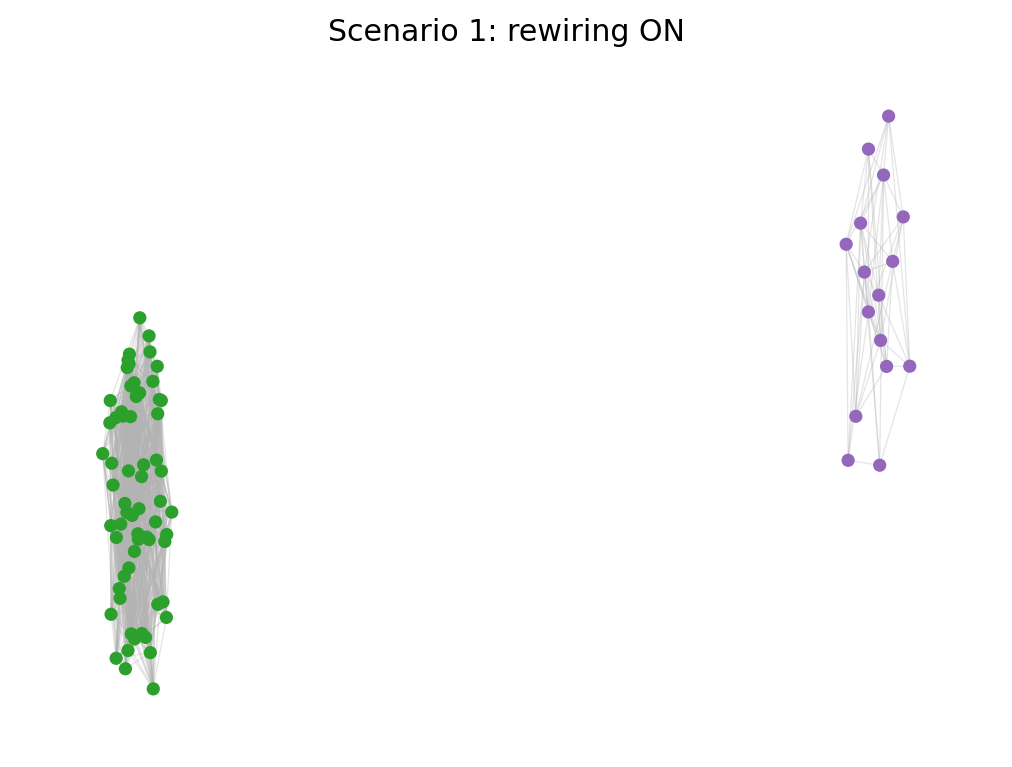
\includegraphics[width=\textwidth]{snapshot_scenario1_rewiring_on.png}
\caption{Rewiring enabled.}
\end{subfigure}\hfill
\begin{subfigure}{0.48\textwidth}
\centering
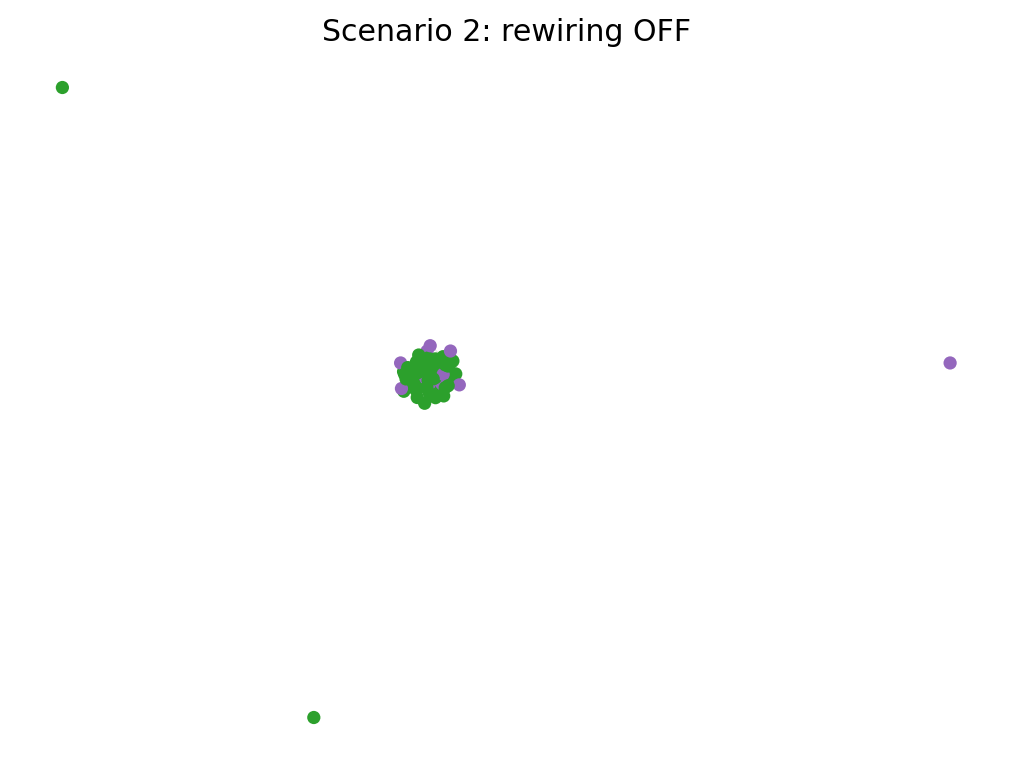
\includegraphics[width=\textwidth]{snapshot_scenario2_rewiring_off.png}
\caption{Rewiring disabled.}
\end{subfigure}
\caption{Baseline network snapshots generated from the first Python prototype. Node colours distinguish hosts and guests; the comparison illustrates the qualitative effect of adaptive rewiring on the final topology.}
\label{fig:baseline-snapshots}
\end{figure}

Figure~\ref{fig:advanced-snapshots} gives the corresponding output of the revised package for the three topologies. Node colour represents the neutrosophic score and node size is proportional to degree, making hubs and potential cultural brokers visually apparent.

\begin{figure}[H]
\centering
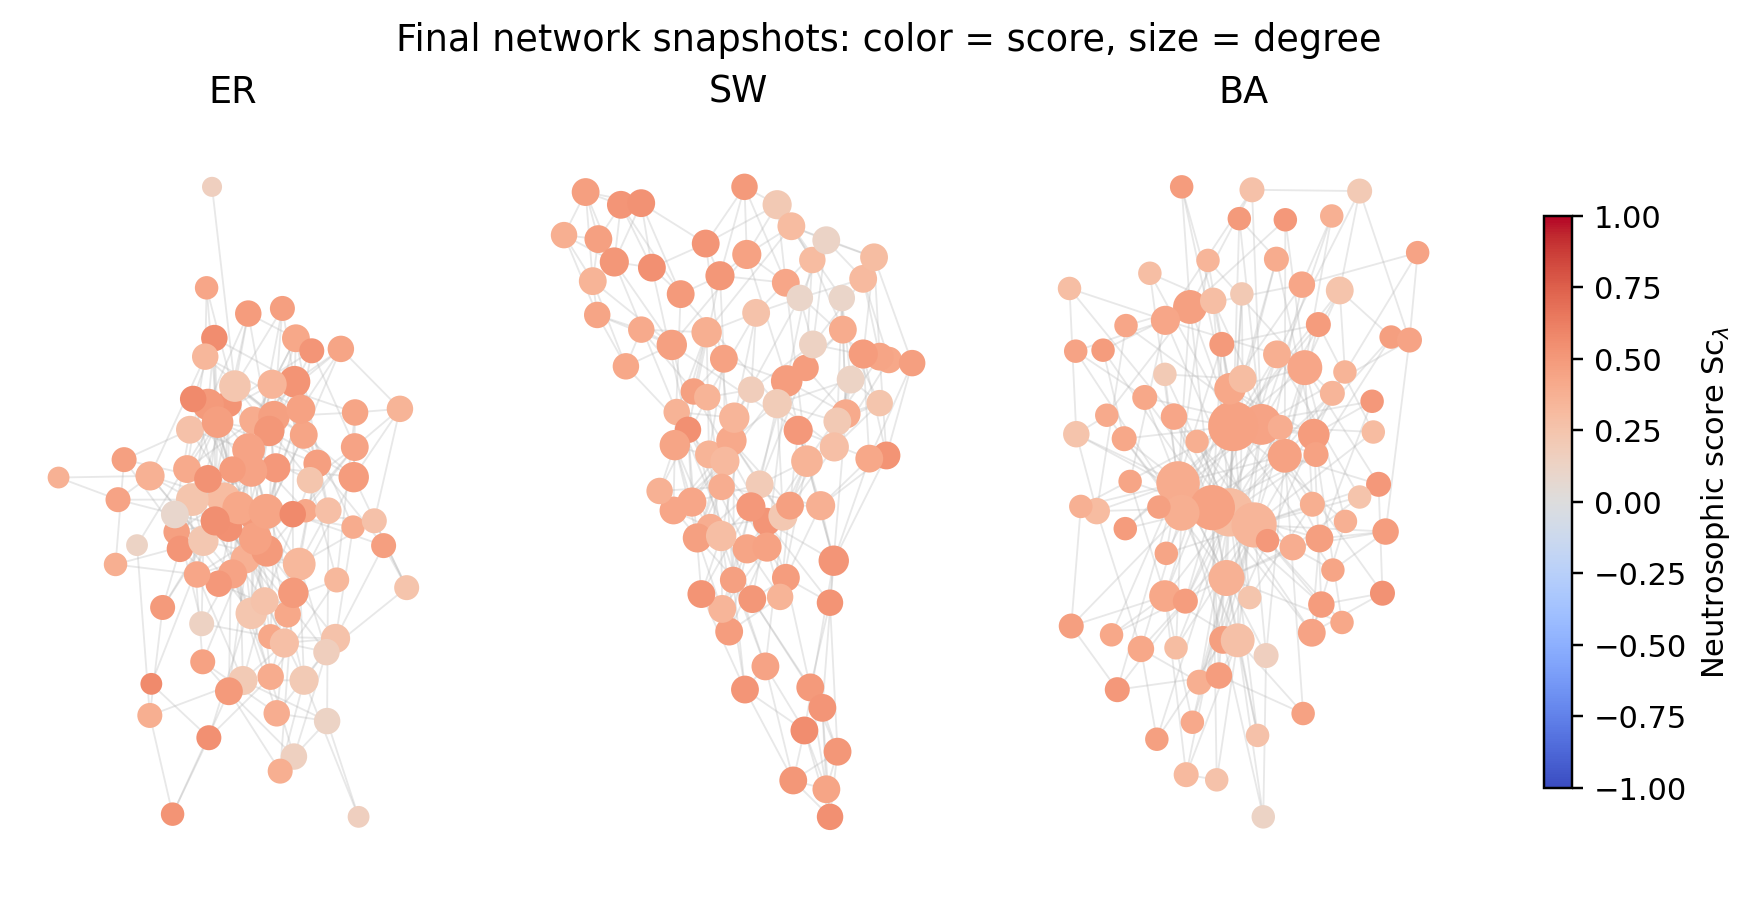
\includegraphics[width=0.95\textwidth]{fig_network_snapshots.png}
\caption{Final network snapshots generated by the revised implementation for ER, SW, and BA topologies. Node colour encodes $\operatorname{Sc}_{\lambda}$ and node size encodes degree.}
\label{fig:advanced-snapshots}
\end{figure}

	\subsection{Erd\H{o}s--R\'enyi vs. Small-World vs. Scale-Free}	Figure~\ref{fig:topology-metrics} compares the integration index $I_{\mathrm{int}}$ and the cross-group reward share $v_{\mathrm{out}}$ under the three network families. The scale-free case is especially relevant because the presence of hubs can either accelerate integration or consolidate enclaves depending on the sign of cross-group reward and trust.
	
	\begin{figure}[H]
		\centering
		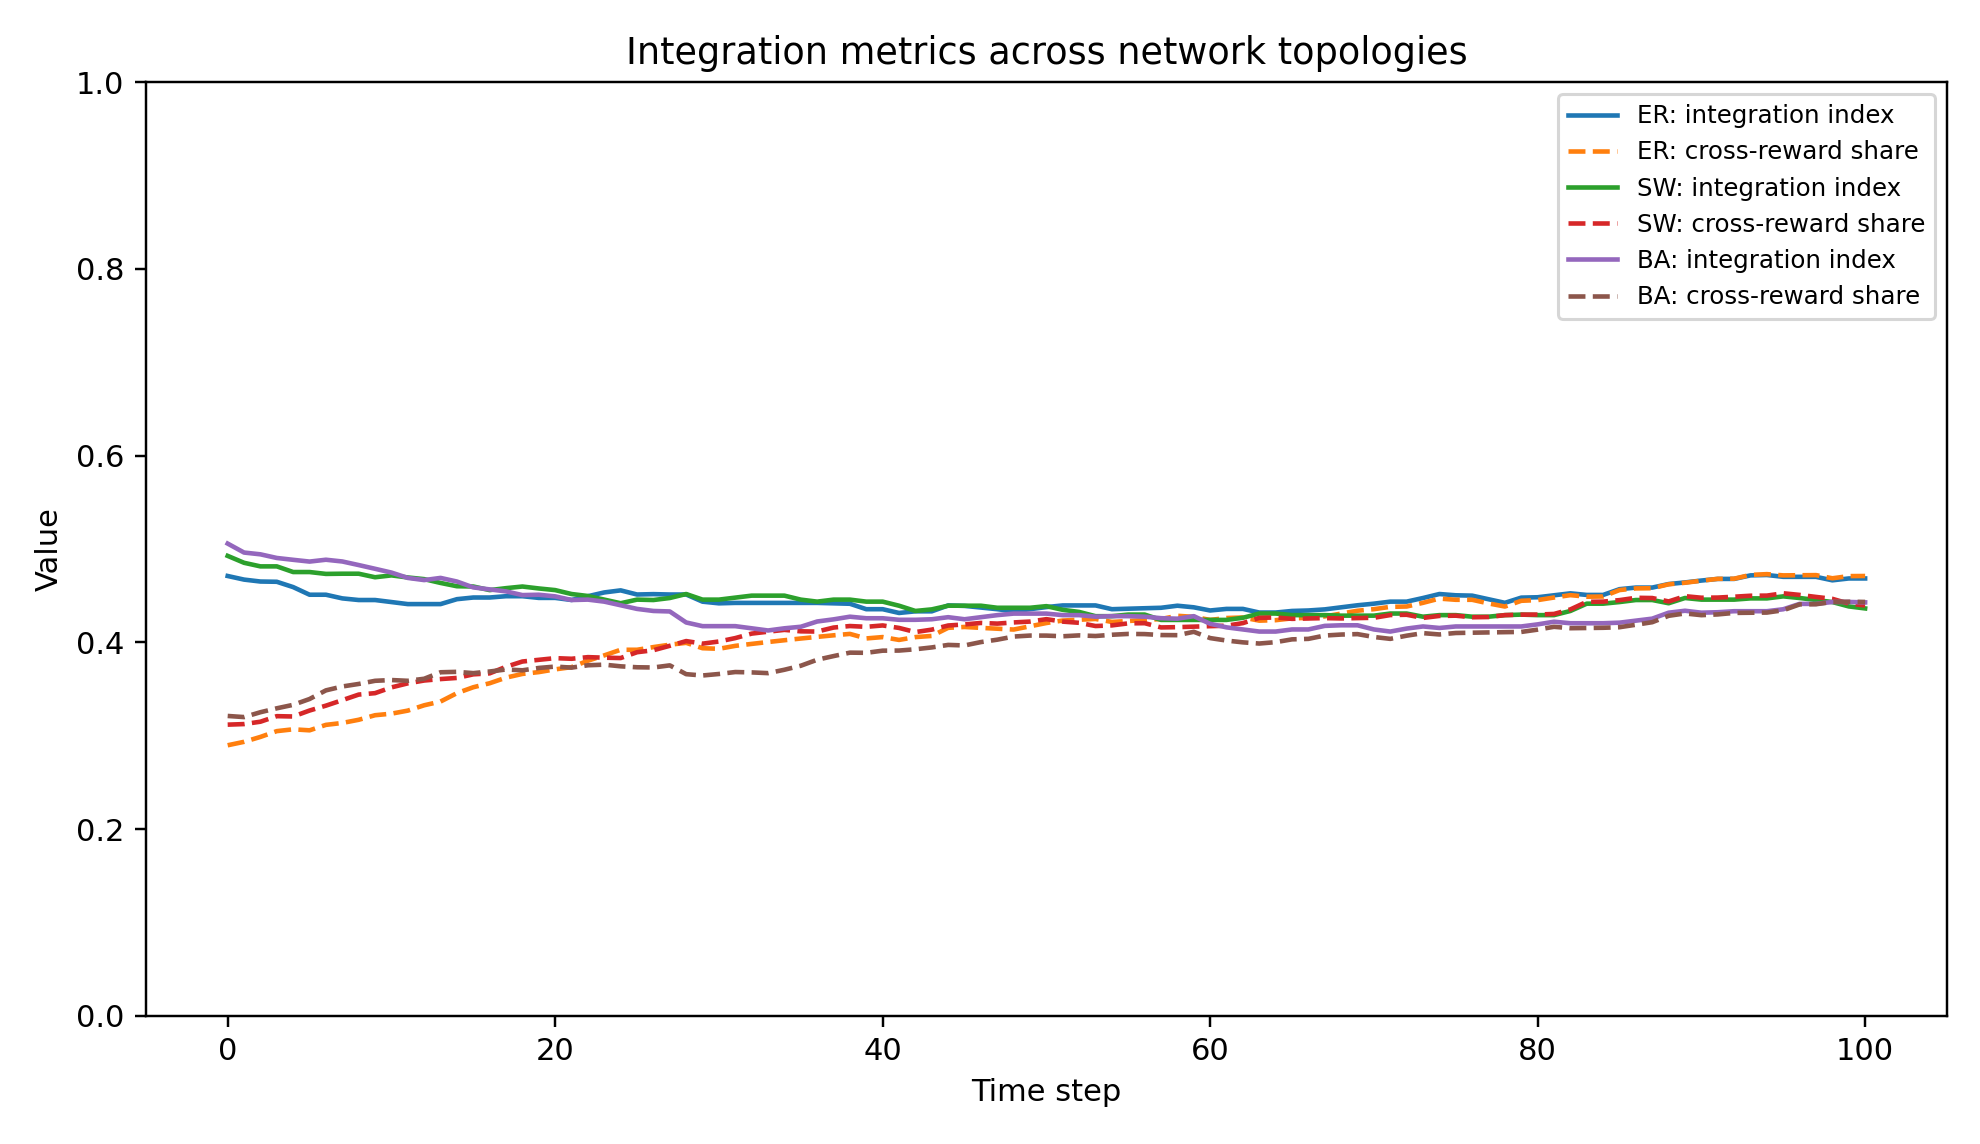
\includegraphics[width=0.92\textwidth]{fig_topology_metrics.png}
		\caption{Integration metrics for Erd\H{o}s--R\'enyi (ER), small-world (SW), and Barab\'asi--Albert scale-free (BA) topologies. Solid curves show $I_{\mathrm{int}}$; dashed curves show $v_{\mathrm{out}}$.}
		\label{fig:topology-metrics}
	\end{figure}
	
	\begin{table}[H]
		\centering
		\small
		\caption{Final aggregate indicators in the three simulated scenarios. Average path length is computed on the largest connected component when the final graph is not connected.}
		\label{tab:summary}
		\begin{tabular}{lcccccc}
			\toprule
			Scenario & $I_{\mathrm{int}}$ & $v_{\mathrm{out}}$ & Integrator & Clustering & Avg. path & Score gap \\
			\midrule
			ER & 0.468 & 0.471 & 0.350 & 0.091 & 2.730 & 0.114 \\
			SW & 0.436 & 0.439 & 0.334 & 0.175 & 2.896 & 0.122 \\
			BA & 0.443 & 0.443 & 0.347 & 0.110 & 2.687 & 0.122 \\
			\bottomrule
		\end{tabular}
	\end{table}
	
	In this representative run, the small-world topology has the strongest local clustering, while the scale-free topology has the shortest effective paths. The final integration levels are comparable, but the mechanisms differ. In small-world networks, integration depends on weak bridges between clusters. In scale-free networks, integration depends on whether hubs become cross-group brokers or intra-group attractors.
	
	\subsection{Integrator index over time}
	Figure~\ref{fig:integrator-evolution} tracks the mean value of the ten largest integrator indices. This quantity combines betweenness, cross-group exposure, and neutrosophic compatibility. It is more informative than degree alone because a high-degree agent inside a homogeneous enclave is not an integrator.
	
	\begin{figure}[H]
		\centering
		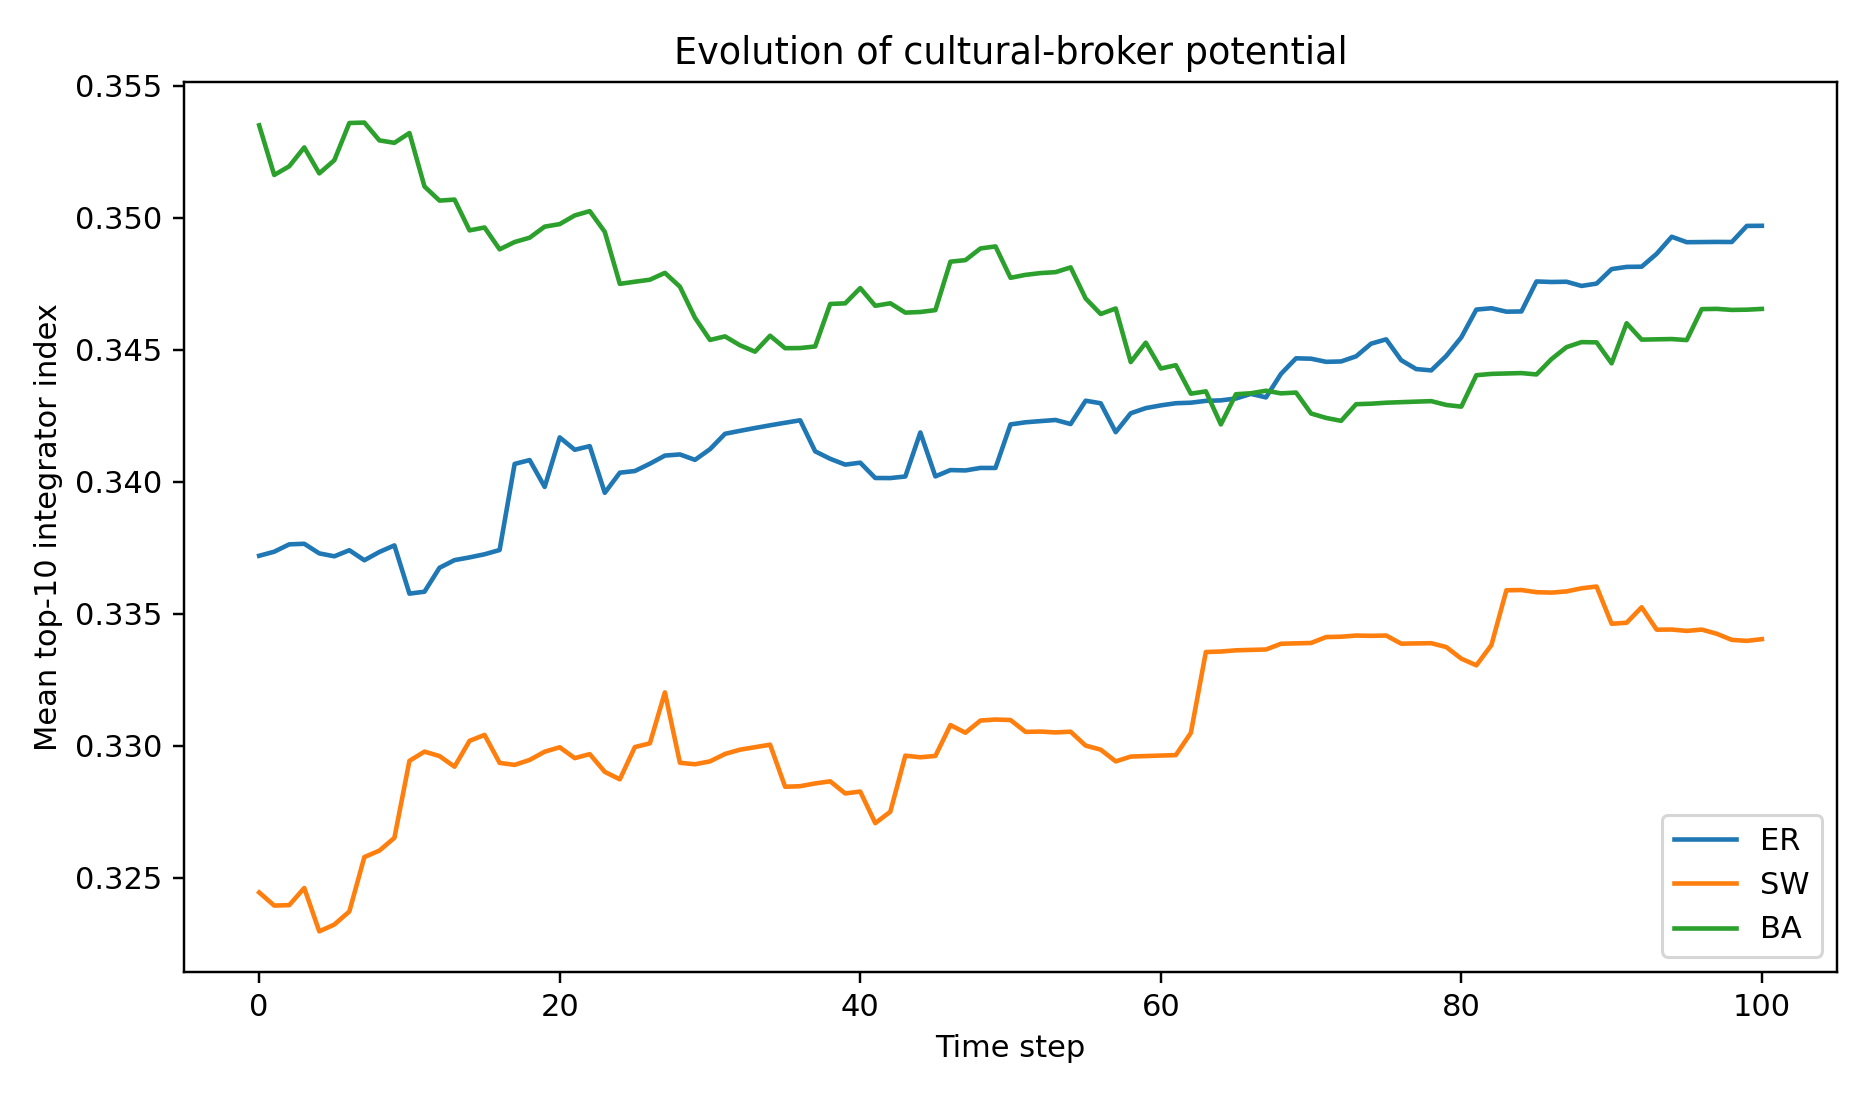
\includegraphics[width=0.88\textwidth]{fig_integrator_evolution.png}
		\caption{Evolution of cultural-broker potential. The plotted quantity is the mean of the ten largest values of the integrator index $\mathcal{B}^t(i)$.}
		\label{fig:integrator-evolution}
	\end{figure}
	
	\subsection{Structural signatures}
	Figure~\ref{fig:topology-structure} reports the final clustering coefficient and average path length. These structural indicators explain why topologies with similar $I_{\mathrm{int}}$ may have different resilience. A clustered network can preserve local stability after a shock, but it may also preserve local segregation. A scale-free network transmits shocks quickly through hubs; this can be beneficial if hubs are integrators and harmful if hubs are enclave leaders.
	
	\begin{figure}[H]
		\centering
		
\includegraphics[width=0.88\textwidth]{fig_topology_structure.png}
		\caption{Structural signatures of the final networks. Clustering measures local closure; average path length measures global reachability.}
		\label{fig:topology-structure}
	\end{figure}
	
	\subsection{Centrality table: scale-free cultural brokers}
	Table~\ref{tab:centrality} reports the agents with the highest integrator index in the final scale-free network. The most relevant agents are not simply those with the highest score: they combine degree, cross-group exposure, betweenness, and closeness.
	
	\begin{table}[H]
		\centering
		\scriptsize
		\caption{Top cultural brokers in the final scale-free network.}
		\label{tab:centrality}
		\begin{tabular}{r l r c c c c c c}
			\toprule
			Node & Group & Degree & Score & NDC & NCC & Betweenness & Cross-share & $\mathcal{B}$ \\
			\midrule
			3 & guest-2 & 16 & 0.260 & 0.178 & 0.461 & 0.087 & 0.875 & 0.381 \\
			0 & guest-2 & 17 & 0.261 & 0.189 & 0.468 & 0.104 & 0.765 & 0.363 \\
			82 & guest-1 & 7 & 0.336 & 0.078 & 0.380 & 0.011 & 1.000 & 0.349 \\
			10 & guest-1 & 14 & 0.297 & 0.155 & 0.459 & 0.065 & 0.786 & 0.346 \\
			19 & guest-1 & 5 & 0.211 & 0.056 & 0.385 & 0.004 & 1.000 & 0.342 \\
			7 & guest-2 & 5 & 0.335 & 0.056 & 0.379 & 0.006 & 1.000 & 0.341 \\
			76 & guest-2 & 4 & 0.346 & 0.045 & 0.363 & 0.009 & 1.000 & 0.337 \\
			35 & guest-1 & 3 & 0.240 & 0.033 & 0.384 & 0.002 & 1.000 & 0.336 \\
			\bottomrule
		\end{tabular}
	\end{table}
	
	The table illustrates the analytical value of neutrosophic centrality. Agents with high cross-share and high closeness may be effective integrators even when their degree is moderate. Conversely, high-degree nodes must be evaluated through their cross-group reward and trust profile before they are interpreted as positive opinion leaders.
	
	\subsection{Neighbourhood tipping}
	Figure~\ref{fig:tipping} shows a tipping experiment in which the migrant fraction is varied and the small-world topology is held fixed. The final integration index is compared with the host--migrant score gap. A tipping warning occurs when the score gap remains high while integration drops below a prescribed level.
	
	\begin{figure}[H]
		\centering
		
\includegraphics[width=0.88\textwidth]{fig_tipping.png}
		\caption{Neighbourhood tipping experiment under small-world topology. The migrant fraction is varied and the model records final integration and final host--migrant score gap.}
		\label{fig:tipping}
	\end{figure}
	
	The illustrative run does not imply a universal critical fraction. Rather, it shows how the model can estimate a context-dependent threshold $\phi_c(\mathcal{T})$ once rewards, trust, initial attitudes, and policy parameters are calibrated. This is methodologically important: collapse toward segregation is not caused by population share alone, but by a feedback loop among density, low trust, high attitudinal distance, and link deletion.
	
	\subsection{Discussion: resilience and external shocks}
	The comparison suggests that topology affects not only the speed of convergence, but also resilience to external shocks. In an Erd\H{o}s--R\'enyi network, shocks are dispersed across a relatively homogeneous random structure. In a small-world network, local clusters can absorb shocks without immediately affecting the whole network, but the same clustering may preserve segregated attitudes. In a scale-free network, hubs make the system highly sensitive to targeted interventions: supporting integrator hubs can accelerate convergence, while the loss or radicalization of a hub can rapidly reduce cross-group cohesion.
	
	The neutrosophic representation makes this distinction more visible. A scalar model may register only a shift in mean attitude, whereas the triple $\nstriple{T,I,F}$ distinguishes increased integration $T$, persistent rejection $F$, and transitional uncertainty $I$. In policy terms, this matters because an intervention may not immediately convert rejection into acceptance; it may first increase indeterminacy, hesitation, or openness. The model can therefore represent a pre-integration phase that scalar models tend to hide.
	
	\section{Conclusions and future perspective}
	We have strengthened the mathematical and methodological basis of a neutrosophic agent-based model for immigration and coexistence while preserving the SVNS framework $\nstriple{T,I,F}$. The revised model compares Erd\H{o}s--R\'enyi, small-world, and scale-free topologies; introduces capacity-dependent utility; replaces myopic rewiring by Q-learning and DSmT-inspired trust aggregation; allows multiple migrant groups and asymmetric relational strength; and defines centrality-based integrator indices. Numerical illustrations show how topology changes the interpretation of integration: small-world networks emphasize weak bridges between cohesive clusters, whereas scale-free networks emphasize the role of hubs. Finally, the tipping experiment provides a way to estimate when a demographic and attitudinal configuration becomes unstable and shifts toward enclave segregation.

\section*{Code availability}
The Python implementation accompanying this article is provided as a reproducibility package. It contains the package \texttt{nsimmigration}, scripts for reproducing all figures, and a README with instructions for creating the public GitHub repository \texttt{giorgionordo/neutrosophic-immigration-model}.

\section*{Acknowledgements}
	This research was supported by Gruppo Nazionale per le Strutture Algebriche, Geometriche e le loro Applicazioni (G.N.S.A.G.A.) of Istituto Nazionale di Alta Matematica (INdAM) ``F.~Severi'', Italy.
	
	\begin{thebibliography}{99}
		
		\bibitem{alam2012} Alam S.J., Tsvetovat M. \textit{Networks in Agent-Based Social Simulation}. Springer, 2012.
		
		\bibitem{barabasi1999} Barab\'asi A.-L., Albert R. Emergence of scaling in random networks. \textit{Science}, vol. 286, no. 5439, pp. 509--512, 1999.
		
		\bibitem{barrat2008} Barrat A., Barth\'elemy M., Vespignani A. \textit{Dynamical Processes on Complex Networks}. Cambridge University Press, 2008.
		
		\bibitem{benczik2009adaptive} Benczik I.J., Benczik S.Z., Schmittmann B., Zia R.K.P. Opinion dynamics on an adaptive random network. \textit{Physical Review E}, vol. 79, 046104, 2009.
		
		\bibitem{broumi2016} Broumi S., Talea M., Bakali A., Smarandache F. Single valued neutrosophic graphs. \textit{Journal of New Theory}, vol. 10, pp. 86--101, 2016.
		
		\bibitem{chen2020marl} Chen Y., Hu Y., Huang S., et al. Social structure emergence: A multi-agent reinforcement learning framework. \textit{Proceedings of AAMAS}, pp. 1807--1809, 2020.
		
		\bibitem{chuang2019} Chuang Y.-L., Chou T., D'Orsogna M.R. A network model of immigration: Enclave formation vs. cultural integration. \textit{Networks and Heterogeneous Media}, vol. 14, no. 1, pp. 53--77, 2019.
		
		\bibitem{chuang2020} Chuang Y.-L., Chou T., D'Orsogna M.R. A network model of immigration and coexistence. \textit{SIAM News}, vol. 53, no. 3, 2020.
		
		\bibitem{dezert2004fusion} Dezert J., Smarandache F. Fusion of imprecise, uncertain, and conflicting beliefs with DSm rules of combination. \textit{arXiv:math/0404305}, 2004.
		
		\bibitem{dezert2006dsmt} Dezert J., Smarandache F. DSmT: A new paradigm shift for information fusion. \textit{arXiv:cs/0610175}, 2006.
		
		\bibitem{freeman1977} Freeman L.C. A set of measures of centrality based on betweenness. \textit{Sociometry}, vol. 40, no. 1, pp. 35--41, 1977.
		
		\bibitem{ganati2023turiyam} Ganati G.A. Relations in the context of Turiyam sets. \textit{Journal of Mathematics}, 2023.
		
		\bibitem{gross2007adaptive} Gross T., Blasius B. Adaptive coevolutionary networks: a review. \textit{Journal of the Royal Society Interface}, vol. 5, no. 20, pp. 259--271, 2007.
		
		\bibitem{haw2017} Haw D.J., Hogan S.J. A dynamical systems model of unorganized segregation. \textit{arXiv preprint} arXiv:1709.07568, 2017.
		
		\bibitem{hui2020} Hui Y., Dey A. A Study on Directed Neutrosophic Social Networks. \textit{IAENG International Journal of Applied Mathematics}, vol. 50, no. 2, pp. 1--8, 2020.
		
		\bibitem{kan2023adaptive} Kan U., Feng M., Porter M.A. An adaptive bounded-confidence model of opinion dynamics on networks. \textit{Journal of Complex Networks}, vol. 11, no. 1, cnac055, 2023.
		
		\bibitem{kandasamy2015} Kandasamy W.B.V., Ilanthenral K., Smarandache F. \textit{Neutrosophic Graphs: A New Dimension to Graph Theory}. EuropaNova ASBL, 2015.
		
		\bibitem{mahapatra2020}
		Mahapatra R., Samanta S., Pal M., Xin Q. Link prediction in social networks by neutrosophic graph. 
		\textit{International Journal of Computational Intelligence Systems}, vol. 13, no. 1, pp. 1699--1713, 2020. 
		doi:10.2991/ijcis.d.201015.002.
		
		\bibitem{newman2010} Newman M.E.J. \textit{Networks: An Introduction}. Oxford University Press, 2010.
		
		\bibitem{peng2022}
		Peng J., Tian C. A large-scale group decision-making method based on single-valued neutrosophic information under the social network environment. 
		\textit{Journal of Systems Science and Mathematical Sciences}, vol. 42, no. 4, pp. 935--954, 2022. 
		doi:10.12341/jssms21314.
		
		\bibitem{schelling1969} Schelling T.C. Models of segregation. \textit{American Economic Review}, vol. 59, no. 2, pp. 488--493, 1969.
		
		\bibitem{schelling1971} Schelling T.C. Dynamic models of segregation. \textit{Journal of Mathematical Sociology}, vol. 1, no. 2, pp. 143--186, 1971.
		
		\bibitem{smarandache1999} Smarandache F. \textit{A Unifying Field in Logics. Neutrosophy: Neutrosophic Probability, Set and Logic}. Rehoboth: American Research Press, 1999.
		
		\bibitem{smarandache2020totalorder} Smarandache F. The Score, Accuracy, and Certainty Functions determine a Total Order on the Set of Neutrosophic Triplets $(T,I,F)$. \textit{Neutrosophic Sets and Systems}, vol. 38, pp. 1--14, 2020.
		
		\bibitem{sodenkamp2018}
		Sodenkamp M.A., Tavana M., Di Caprio D. An aggregation method for solving group multi-criteria decision-making problems with single-valued neutrosophic sets. 
		\textit{Applied Soft Computing}, vol. 71, pp. 715--727, 2018. 
		doi:10.1016/j.asoc.2018.07.020.
		
		\bibitem{sutton2018} Sutton R.S., Barto A.G. \textit{Reinforcement Learning: An Introduction}. 2nd ed., MIT Press, 2018.
		
		\bibitem{wang2010svns} Wang H., Smarandache F., Zhang Y.Q., Sunderraman R. Single Valued Neutrosophic Sets. \textit{Technical Sciences and Applied Mathematics}, pp. 10--14, 2010.
		
		\bibitem{watkins1992} Watkins C.J.C.H., Dayan P. Q-learning. \textit{Machine Learning}, vol. 8, pp. 279--292, 1992.
		
		\bibitem{watts1998} Watts D.J., Strogatz S.H. Collective dynamics of small-world networks. \textit{Nature}, vol. 393, pp. 440--442, 1998.
		
		\bibitem{yang2016} Yang H.-L., Guo Z.-L., She Y., Liao X. On single valued neutrosophic relations. \textit{Journal of Intelligent \& Fuzzy Systems}, vol. 30, no. 2, pp. 1045--1056, 2016.
		
		\bibitem{ye2012} Ye D., Zhang M., Sutanto D. Self-organization in an agent network: A mechanism and a potential application. \textit{Decision Support Systems}, vol. 53, no. 3, pp. 406--417, 2012.
		
		\bibitem{ye2014crossentropy}
		Ye J. Single-valued neutrosophic cross-entropy for multicriteria decision-making problems. 
		\textit{Applied Mathematical Modelling}, vol. 38, no. 3, pp. 1170--1175, 2014. 
		doi:10.1016/j.apm.2013.07.020.
		
	\end{thebibliography}
	
\end{document}
